\documentclass[12pt,a4paper]{article}

% -------------------------------------------------
% Codificación e idioma
% -------------------------------------------------
\usepackage[T1]{fontenc}
\usepackage[utf8]{inputenc}
\usepackage[english,spanish,es-tabla,es-nodecimaldot]{babel}

% -------------------------------------------------
% Página y tipografía
% -------------------------------------------------
\usepackage[a4paper,left=2cm,right=2cm,top=2.25cm,bottom=2.25cm]{geometry}
\usepackage{microtype}
\usepackage{newtxtext,newtxmath} % Times-like, más estable que mezclar con cmbright

% -------------------------------------------------
% Matemáticas y unidades
% -------------------------------------------------
\usepackage{mathtools}
\usepackage{amsmath}
%\usepackage{amssymb}
\usepackage{physics}
\usepackage{siunitx}

\sisetup{
  output-decimal-marker = {.},
  exponent-mode         = threshold,
  exponent-thresholds   = -4:5,
  round-mode            = uncertainty,
  round-precision       = 2,
  print-unity-mantissa  = false,
  inter-unit-product    = \ensuremath{{}\cdot{}},
  inline-per-mode       = single-symbol,
  display-per-mode      = fraction,
  separate-uncertainty = true
}

% -------------------------------------------------
% Figuras y tablas
% -------------------------------------------------
\usepackage{graphicx}
\usepackage{booktabs}
\usepackage{caption}
\captionsetup{
  font=small,
  justification=centerlast,
  skip=6pt,
  labelfont={bf,small},
  textfont={small}
}

% -------------------------------------------------
% Colores e hipervínculos
% -------------------------------------------------
\usepackage[dvipsnames]{xcolor}
\usepackage{hyperref}
\hypersetup{
  colorlinks=true,
  linkcolor=Blue,
  citecolor=ForestGreen,
  urlcolor=BrickRed,
  pdftitle={Centelleo en la mezcla gaseosa Ar--N2},
  pdfauthor={Daniel Vázquez Lago}
}

% -------------------------------------------------
% Bibliografía
% -------------------------------------------------
\usepackage{csquotes}
\usepackage[
  backend=biber,
  style=numeric,
  sorting=none
]{biblatex}
\addbibresource{sample.bib}

% ------------------------------------------------
% Encabezados y pies
% -------------------------------------------------
\usepackage{fancyhdr}
\pagestyle{fancy}
\fancyhf{}
\fancyhead[L]{Trabajo de Fin de Máster}
\fancyhead[R]{Daniel Vázquez Lago}
\fancyfoot[R]{\thepage}
\renewcommand{\headrulewidth}{0.4pt}
\renewcommand{\footrulewidth}{0pt}


% -------------------------------------------------
% Rutas de figuras
% -------------------------------------------------
\graphicspath{
  {experimental_espectra/}
  {cross_sections/}
  {kinetic_models/}
  {garfield++/}
  {primary_fit/}
  {secondary_fit/}
  {prediction_plots/}
  {spectra/}
}

\renewcommand{\arraystretch}{1.40}
% -------------------------------------------------
% Macros matemáticas
% -------------------------------------------------
\newcommand{\N}{\mathrm{N}}
\newcommand{\He}{\mathrm{He}}
\newcommand{\Ar}{\mathrm{Ar}}
\newcommand{\CF}{\mathrm{CF}}
\newcommand{\NC}{\mathrm{N}_2^*(\mathrm{C})}
\newcommand{\norma}{\mathrm{norm}}
\newcommand{\vis}{\mathrm{vis}}
\newcommand{\uv}{\mathrm{uv}}
\newcommand{\third}{\mathrm{3rd}}
\newcommand{\dir}{\mathrm{dir}}
\newcommand{\phe}{\mathrm{ph/e^-}}
\newcommand{\vib}{\mathrm{v}}
\newcommand{\nm}{\mathrm{nm}}
\newcommand{\threshold}{\mathrm{threshold}}
\newcommand{\scint}{\mathrm{scint}}

% Versiones robustas para títulos
\DeclareRobustCommand{\Nt}{\ensuremath{\mathrm{N}_2}}
\DeclareRobustCommand{\CFt}{\ensuremath{\mathrm{CF}_4}}
\DeclareRobustCommand{\Argas}{\ensuremath{\mathrm{Ar}}}
\DeclareRobustCommand{\ArN}{\ensuremath{\mathrm{Ar}-\mathrm{N}_2}}

% Estados útiles para evitar Unicode raro tipo ¹s4
\DeclareRobustCommand{\ArOneSFour}{\ensuremath{\mathrm{Ar}^*(1s_4)}}
\DeclareRobustCommand{\ArOneSFive}{\ensuremath{\mathrm{Ar}^*(1s_5)}}

% -------------------------------------------------
% Documento
% -------------------------------------------------
\begin{document}
\selectlanguage{spanish}

% -------------------------
% Portada
% -------------------------
\thispagestyle{empty}
\begin{titlepage}
    \centering
    \vspace*{0.20\textheight}

    {\Huge\bfseries Trabajo de Fin de Máster\par}
    \vspace{2.2em}

    {\LARGE\bfseries Centelleo en la Mezcla Gaseosa $\Ar-\N_2$\par}
    \vspace{5em}

    {\Large Daniel Vázquez Lago\par}
    \vspace{2.2em}

    {\Large \today\par}
\end{titlepage}

% -------------------------
% Índice
% -------------------------
\pagestyle{empty}
\tableofcontents
\clearpage

% -------------------------------------------------
% Formato de párrafo
% -------------------------------------------------
\setlength{\parindent}{0pt}
\setlength{\parskip}{0.45em}

\pagestyle{fancy}

\section{Introducción}

La detección de partículas es uno de los pilares experimentales de la física moderna. La información física de un proceso microscópico no se obtiene de forma directa, sino a través de las huellas que dejan las partículas al atravesar la materia: ionización, excitación, centelleo, desplazamiento de carga, producción de calor o emisión de radiación secundaria. En función de cuál de estos observables se quiera privilegiar, y de las condiciones experimentales de cada problema, se han desarrollado familias de detectores muy distintas entre sí. Los detectores de silicio dominan hoy en día los entornos de muy alta ocupación y gran resolución espacial; los calorímetros permiten medir energía y topología de chorros o cascadas; y los detectores basados en gases y en medios nobles continúan siendo una solución especialmente competitiva cuando se buscan grandes volúmenes activos, baja masa material, buena capacidad de imagen y costes razonables por unidad de superficie. En este panorama, el estado del arte no está marcado por una única tecnología, sino por la convivencia de soluciones muy especializadas, optimizadas para necesidades instrumentales diferentes.

\subsection{Detectores Gaseosos}

Dentro de ese ecosistema, los detectores gaseosos mantienen una posición singular. Su principio de funcionamiento es conceptualmente simple: una partícula cargada o una radiación ionizante deposita energía en el gas, crea pares electrón--ión y estados excitados, y la señal se forma a partir del transporte de esas cargas o de la luz emitida durante la excitación y la avalancha. Sin embargo, detrás de esa idea sencilla hay una enorme riqueza instrumental. La composición del gas, la presión, la geometría del detector y el campo eléctrico permiten modular de manera fina la deriva, la difusión, la ganancia, la tasa de \textit{attachment} y la producción de luz. Por ello, los detectores gaseosos siguen siendo una herramienta de referencia en trazado, identificación de partículas, física de neutrinos, búsquedas de procesos raros y detectores de gran volumen 
\cite{gonzlezdaz2017gaseous,hayrapetyan2024dune,next2014present,esfahani2023project}.

En términos históricos, la evolución de los detectores gaseosos puede leerse como una transición desde geometrías macroscópicas, como cámaras de hilos o cámaras proporcionales, hacia estructuras de multiplicación cada vez más finas y controladas. Esa evolución ha respondido a una necesidad muy concreta: reducir la longitud característica de la avalancha para mejorar estabilidad, granularidad, tasa soportada y resolución espacial. En ese contexto aparecen los \emph{micro-pattern gaseous detectors} (MPGDs), que constituyen una de las familias más influyentes en la instrumentación gaseosa contemporánea \cite{shekhtman2002micropattern,buzulutskov2007radiation}. Su importancia no reside solo en haber sustituido en muchos contextos a tecnologías anteriores, sino en haber abierto una vía completamente nueva para combinar multiplicación electrónica, imagen fina y, cada vez más, lectura óptica.

Los MPGDs agrupan dispositivos en los que la amplificación tiene lugar en microestructuras fabricadas con gran precisión: agujeros, mallas o patrones metálicos con dimensiones submilimétricas. Entre los ejemplos más conocidos están los GEM y sus variantes gruesas, como los THGEM, así como otros multiplicadores microestructurados desarrollados para operar en rangos de presión, ganancia o robustez distintos. La ventaja fundamental de estas geometrías es que concentran campos eléctricos intensos en regiones muy pequeñas y bien definidas. Como consecuencia, la avalancha queda más localizada, la respuesta resulta más uniforme, la probabilidad de descarga se controla mejor y la granularidad espacial mejora de manera notable respecto a detectores gaseosos más clásicos \cite{shekhtman2002micropattern,buzulutskov2007radiation,azevedo2016thgem}. Además, la fabricación modular y planar de muchos MPGDs facilita su escalado a áreas grandes y su integración con electrónica segmentada o con sistemas ópticos de lectura.

Desde el punto de vista instrumental, los beneficios de los MPGDs son especialmente atractivos en tres frentes. En primer lugar, permiten trabajar con altas tasas y con patrones de señal muy localizados, algo esencial en experimentos con mucha ocupación o cuando se persigue reconstrucción fina de topologías. Este punto no es solo una ventaja genérica de laboratorio, sino una de las razones por las que los MPGDs han sido adoptados en detectores reales de gran escala. Los GEM de COMPASS demostraron que podían funcionar como trazadores precisos en regiones de alto flujo de partículas; la actualización de la TPC de ALICE sustituyó la lectura proporcional clásica por pilas de GEM para hacer posible la operación en lectura continua a las tasas de interacción de Run 3 y Run 4; y el sistema New Small Wheel de ATLAS emplea Micromegas resistivos en una zona de alto fondo radiativo para proporcionar trazado de precisión y capacidad de disparo en el espectrómetro de muones \cite{ketzer2004compass,adolfsson2021alice,manthos2019atlas}. Estos ejemplos muestran que los MPGDs no son únicamente una tecnología prometedora, sino una solución madura allí donde se necesita combinar granularidad, estabilidad y operación a alta tasa. En segundo lugar, ofrecen una gran versatilidad en la elección de la mezcla gaseosa y de la geometría, lo que permite adaptar el detector a objetivos muy distintos: máxima ganancia, mínima difusión, centelleo intenso o buena resolución temporal. En tercer lugar, los MPGDs son compatibles de forma natural con una lectura híbrida, en la que la misma avalancha puede observarse simultáneamente como carga y como luz. Esa dualidad es una de las razones por las que han pasado de ser simples multiplicadores de carga a convertirse en plataformas muy versátiles para TPCs ópticos, detectores de electroluminiscencia y conceptos avanzados de reconstrucción 3D \cite{oliveira2012simulation,williams2024fatgems}.

\subsection{Centelleo en Detectores Gaseosos}

La utilización del centelleo en MPGDs responde precisamente a esa idea: aprovechar que la avalancha no solo multiplica electrones, sino que también excita especies atómicas y moleculares capaces de emitir fotones. La señal óptica ofrece ventajas que no son redundantes respecto a la carga. En primer lugar, desacopla parcialmente la etapa de amplificación de la de lectura: la información puede recogerse con cámaras, PMTs o SiPMs situados fuera de la zona de alto campo, reduciendo restricciones de cableado y capacitancia. En segundo lugar, la imagen óptica puede proporcionar una granularidad muy alta sobre áreas extensas, especialmente cuando se emplean sensores bidimensionales. En tercer lugar, la luz integra de forma natural información espacial, temporal y topológica: combinada con el tiempo de deriva o con sensores rápidos, permite reconstruir trazas, distinguir morfologías y, en ciertos casos, extraer \emph{timing} absoluto o relativo. Finalmente, en mezclas adecuadas, la emisión puede desplazarse desde el VUV (\textit{Vacuum Ultraviolet}) hacia el UV cercano, el visible o incluso el NIR, regiones donde la fotodetección es tecnológicamente más sencilla y a menudo más barata \cite{bondara2010direct,morozov2012secondary,oliveira2012simulation,santorelli2021spectroscopic,bondar2012study}.

Naturalmente, la lectura por centelleo también introduce limitaciones. La eficiencia óptica total depende no solo del gas, sino de la geometría, del ángulo sólido, de la reflectividad, de las ventanas ópticas y de la eficiencia cuántica o PDE del fotosensor. A diferencia de la carga, la luz puede sufrir pérdidas geométricas importantes y exige una calibración más completa del sistema de detección. Además, la producción de fotones compite con canales no radiativos, con fenómenos de \emph{quenching} colisional y, en determinados gases, con procesos de attachment o de disociación que pueden degradar la linealidad o la estabilidad. En operación a ganancia alta también pueden aparecer efectos de saturación local y de carga espacial en los canales de multiplicación, particularmente relevantes cuando se busca maximizar la salida óptica \cite{christophorou1999electron,amedo2023observation}. En otras palabras, el centelleo en MPGDs no sustituye sin más a la lectura de carga: la complementa, y en algunos escenarios concretos la supera claramente.

A pesar de su interés instrumental, la predicción cuantitativa del centelleo gaseoso sigue siendo un problema mucho menos cerrado que el transporte de carga. Para algunas situaciones concretas sí existen programas experimentales y modelos relativamente desarrollados. Un ejemplo importante procede de la física de rayos cósmicos ultraenergéticos, donde colaboraciones como MACFLY y AIRFLY midieron el rendimiento de fluorescencia de aire seco y N$_2$ puro, así como su dependencia con presión, temperatura, humedad y quenching colisional, con el objetivo de reconstruir la energía de cascadas atmosféricas \cite{colin2007macfly,ave2008airfly}. Sin embargo, ese tipo de descripción está construida para un problema muy específico: fluorescencia de N$_2$ y aire en condiciones atmosféricas, normalmente en el rango UV, excitada por electrones relativistas o por partículas de cascada. No constituye, por tanto, un modelo general capaz de predecir de forma directa el centelleo primario y secundario de mezclas arbitrarias dentro de microestructuras gaseosas sometidas a campos eléctricos intensos.

Esta carencia es especialmente relevante para MPGDs. En un detector óptico real no basta con conocer una sección eficaz de excitación aislada o una banda de emisión concreta. La señal final depende de una cadena de procesos acoplados: producción microscópica de estados excitados e ionizados, transferencia de energía entre especies, recombinación, disociación molecular, \emph{quenching}, formación de excímeros o fragmentos excitados, emisión radiativa, absorción y posible realimentación óptica. Además, en mezclas con gases nobles y moléculas poliatómicas, una misma energía depositada puede redistribuirse entre canales muy diferentes: ionización, excitación atómica, emisión VUV, líneas NIR, bandas moleculares visibles o procesos no radiativos. Por ello, la ausencia de modelos predictivos para mezclas arbitrarias limita de forma directa la optimización de detectores ópticos: impide estimar de antemano cuántos fotones se producirán, en qué rango espectral aparecerán, cómo variarán con presión y concentración, y qué compromisos surgirán entre ganancia, estabilidad, \emph{attachment}, emisión útil y daño por descargas.

El problema no es solo práctico, sino también físico. Un modelo de centelleo suficientemente completo permitiría separar la parte de transporte electrónico, gobernada por las secciones eficaces electrón--gas y por el campo reducido, de la cinética posterior de las especies excitadas. Esa separación es esencial si se quiere extrapolar de una mezcla a otra, interpretar diferencias entre emisión primaria y secundaria, o estudiar efectos que afectan directamente a la medida, como el \emph{photon feedback}, la fotoionización de impurezas o superficies, la aparición de estados metaestables y la competencia entre emisión radiativa y disipación colisional. Desde esta perspectiva, construir un modelo fenomenológico y validarlo frente a datos experimentales no es simplemente una herramienta de ajuste, sino un paso necesario para convertir la lectura óptica de MPGDs en una técnica predictiva y optimizable.


\subsection{¿Por qué Ar--N$_2$?}

La lectura óptica de MPGDs aprovecha la luz emitida durante la producción primaria de excitaciones y durante la avalancha electrónica. Esta estrategia permite observar señales con cámaras, PMTs o SiPMs alejados de la región de alto campo, y puede proporcionar información topológica sobre trazas en TPCs gaseosas. La demostración de centelleo de avalancha en microestructuras y el desarrollo de detectores ópticos muestran que la mezcla gaseosa debe elegirse no solo por deriva y ganancia, sino también por su capacidad de transformar energía depositada en fotones detectables \cite{bondara2010direct,oliveira2012simulation,torelli2022the,williams2024fatgems}.

La mezcla Ar--N$_2$ es especialmente interesante porque combina un gas noble ampliamente utilizado con un aditivo económico, químicamente estable en las condiciones de operación y ambientalmente benigno. Una pequeña fracción de N$_2$ puede recibir energía de estados excitados del argón y emitir en la segunda banda positiva del nitrógeno, situada en el UV cercano y mucho más accesible para la fotodetección convencional que la emisión VUV dominante de un gas noble puro \cite{puech1977energy,morii2004quenching,friedl2012spectral}.

La aparición de emisión del N$_2$ a bajas concentraciones, junto con la reducción de las líneas infrarrojas del argón al aumentar el aditivo, convierte a Ar--N$_2$ en un banco de pruebas limpio para estudiar transferencia de energía, \emph{quenching} y competencia entre canales radiativos. El objetivo de este documento es modelizar esa conversión espectral y obtener predicciones del centelleo primario UV y NIR en función de la concentración y de la presión.


% =================================================
\section{Objetivos}
% =================================================

Este trabajo se centra exclusivamente en el centelleo de la mezcla $\Ar-\N_2$ en regiones de operación relevantes para detectores gaseosos con lectura óptica. El modelo separa la producción microscópica de poblaciones excitadas, calculada mediante Degrad o Garfield++, de su evolución cinética posterior mediante emisión radiativa, transferencia de energía y \emph{quenching} colisional.

Los objetivos concretos son:
\begin{itemize}
    \item Caracterizar las emisiones del argón y del nitrógeno relevantes en el intervalo espectral estudiado, con especial atención a la segunda banda positiva del N$_2$ y a las líneas NIR del Ar.
    \item Construir un modelo cinético para la emisión ultravioleta de $\Ar-\N_2$, incorporando producción directa de $\N_2^*(\mathrm{C})$, transferencia desde estados del argón y desexcitación colisional.
    \item Modelizar la extinción de las líneas NIR del argón en presencia de N$_2$ y extraer los parámetros efectivos correspondientes.
    \item Ajustar el modelo a los datos experimentales en diferentes concentraciones y presiones, propagando por separado incertidumbres estadísticas y sistemáticas.
    \item Obtener predicciones absolutas del centelleo primario UV y NIR y reconstruir espectros esperados en función de la composición y la presión.
    \item Valorar la mezcla $\Ar-\N_2$ como sistema de conversión espectral para detectores ópticos basados en MPGDs.
\end{itemize}

\section{Espectros Experimentales} \label{sec:experimental_espectra}
% =================================================

\subsection{Ar} \label{subsec:Ar_spectra}


El centelleo de los gaases nobles (Ar, Kr, Xe, He, Ne) fue uno de los primeros en ser estudiados por su capacidad de producir bandas espectrales en el VUV, a saber, 126 nm (Ar), 146 nm (Kr) o 178 nm (Xe). En estos primeros estudios se desarrollo el término "segundo continuo" para describir el centelleo observado, ya que no estaba asociado a una transición atómica. En realidad estas emisiones están asociadas a \textit{las transiciones entre excímeros de las diferentes especies}. Un excímero es un dímero (especie química formada por dos molñeculas) en el que uno de los átomos está excitado. En el caso de los gases nobles los excímeros son estables a diferencia de los dímeros. 


\begin{minipage}{0.6\linewidth}
    
Sin embargo, cuando se amplio el dominio de las longitudes de onda se observaron fenómenos no asociables directamente con el segundo continu. A este fenómeno se le denomino \textbf{tercer continuo} (denotado como $X_{\third}$). Hoy en día este tercer continuo se sabe que puede proceder de diferentes especies, tales como $X_2^{+,*}$ o $X_2^{++,(*)}$. . Este fenómeno posee, en función del gas y de la presión, una FWHM de 10 a 100 nm en un rango de 60 a 400 nm. En el caso del argón puede variar desde un pico a 230 nm e 0.5 bar y un pico en 270 nm a 2 bar. En la imagen \ref{fig:3erContinuo} se observa la emisión de cada distinta especie asociada al tercer continuo, así como su posible interacción con otras especies del argon. 

\vspace*{1em}

Otras emisiones en el rango de interés son las emisiones del NIR en el rango de 700-800 nm. Estas lineas están asociadas a transiciones entre multipletes del argon excitado, en particular a las transiciones $3p^5 4p \rightarrow 3p^5 4s$. En la figura \ref{fig:experimentalArGlobalEspectra} podemos observar tanto el tercer continuo y las emisiones del NIR, así como ciertas impurezas procedentes del H$_2$O (310 nm) y N$_2$ (330-410 nm).

\end{minipage} \hfill
\begin{minipage}{0.35\linewidth}
    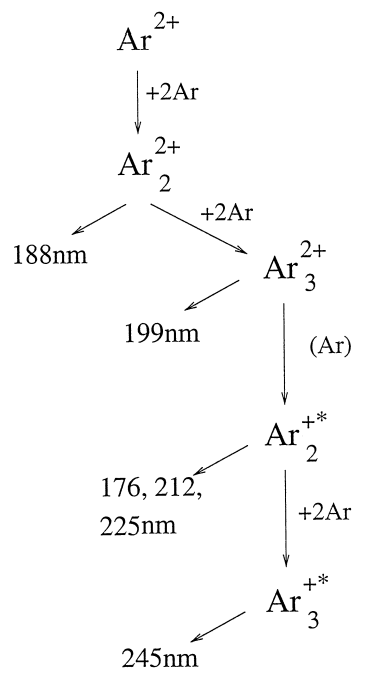
\includegraphics[width=0.8\linewidth]{experimental_espectra/3erContinuo.png} 
    \captionof{figure}{$\Ar_{\third}$ decaimientos \cite{WIESER2000233}.}   
    \label{fig:3erContinuo}
\end{minipage}

\vspace*{1em}

\begin{figure}[htbp]
    \centering
    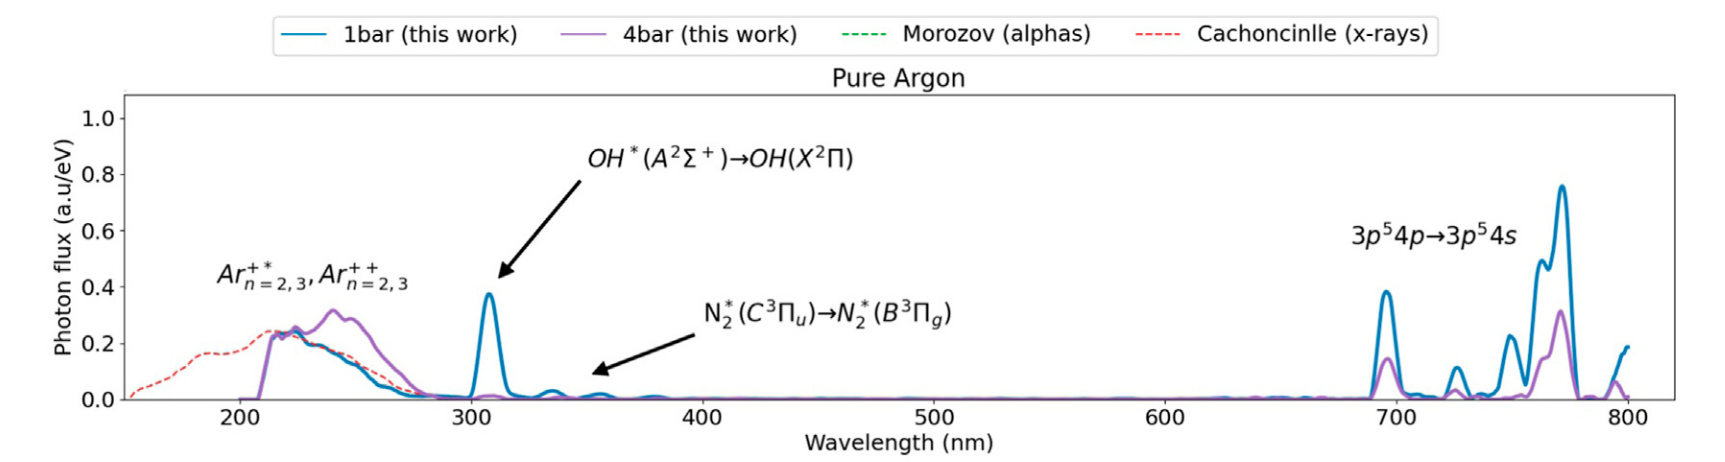
\includegraphics[width=\linewidth]{experimental_espectra/ArEspectroCompleto.png}
    \caption{Espectro experimental 200-800 nm por rayo X en argón puro \cite{amedo2023observation}.}
    \label{fig:experimentalArGlobalEspectra}
\end{figure} 

Como ya hemos dicho, en la región del infrarrojo cercano (NIR), el argón emite varias líneas atómicas asociadas a transiciones \(3p^5 4p \rightarrow 3p^5 4s\), descritas en la notación de Paschen como \(2p_n \rightarrow 1s_m\). En nuestro rango de estudio será especialmente relevante las transiciones de la tabla \ref{tab:ArNIRlines}. 

\begin{table}[htbp]
    \centering
    \caption{Principales líneas NIR del argón consideradas en este trabajo \cite{Wiese1989Argon}.}
    \label{tab:ArNIRlines}
    \begin{tabular}{cccc}
        \toprule
        $\lambda$ (nm) & Transición & $\tau$ [ns] \\
        \midrule
        696 & $2p_2 \rightarrow 1s_5$ & 28.3 \\
        727 & $2p_2 \rightarrow 1s_4$ & 28.3 \\
        750 & $2p_1 \rightarrow 1s_2$ & 21.7 \\
        763 & $2p_6 \rightarrow 1s_5$ & 29.4 \\
        772 & $2p_2 \rightarrow 1s_3$ & 28.3 \\
        794 & $2p_4 \rightarrow 1s_3$ & 29.4 \\
        \bottomrule
    \end{tabular}
\end{table}


\subsection{N$_2$}

El dinitrógeno o N$_2$ es un gas ecológico, inerte químicamente y extremadamente barato, por lo que es un buen candidato a sustituir el \CFt, un compuesto con un alto impacto medioambiental. Su emisión más prominente en el rango de presiones y espectro estudiadas, es
$$ \N_2 (\mathrm{C}^3\Pi_u) \rightarrow \N_2  (\mathrm{B}^3\Pi_g) + h \nu (260-430\mathrm{nm}) $$
llamado 2º banda positiva del $\NC$. El $\NC$ tiene 4 estados en vibracionales, mientras que el $\N_2(\mathrm{B})$ posee hasta 16 estados vibracionales. Las emisiones más predominantes suceden entre los estados vibracionales más bajos del $\NC$ hacia los estados vibracionales más bajos del $\N_2(\mathrm{B})$. Véase imágenes \ref{fig:N2_spectra} y \ref{fig:N2_potential}. En particular, en el rango de presiones y concentraciones de interés, los decaimientos observables son: 

$$ \N_2 (\mathrm{C}^3\Pi_u, v = 0) \rightarrow  (\mathrm{B}^3\Pi_g, v=0,1,2,3) + h \nu (338,358,380,408 \ \mathrm{nm})  $$


\begin{minipage}{0.48\linewidth}
    \centering
    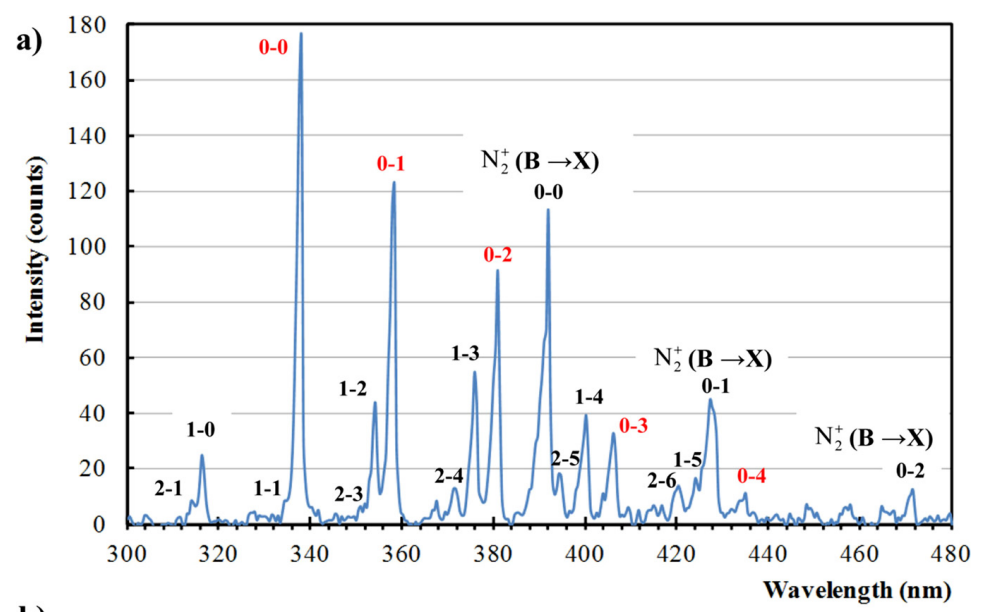
\includegraphics[width=0.99\linewidth]{experimental_espectra/N2_spectra.png}
    \captionof{figure}{Emisión del $\N_2$ \cite{Bayram2012}.}
    \label{fig:N2_spectra}
\end{minipage}
\hfill
\begin{minipage}{0.48\linewidth}
    \centering
    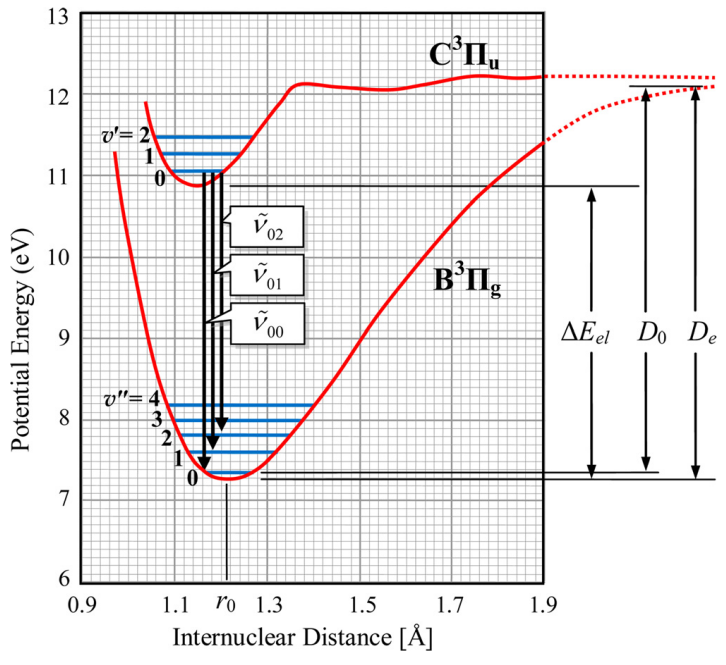
\includegraphics[width=0.7\linewidth]{experimental_espectra/N2_potential.png}   
    \captionof{figure}{Curvas de potencial  $\N_2 (\mathrm{C}), \N_2  (\mathrm{B})$  \cite{Bayram2012}.} 
    \label{fig:N2_potential}
\end{minipage}

\subsection{Ar--N$_2$}

Una vez identificadas las emisiones individuales de Ar y N$_2$, la mezcla permite observar el efecto de la transferencia energética entre ambas especies. En la figura~\ref{fig:experimentalArN2GlobalEspectra} la segunda banda positiva del nitrógeno aparece ya para concentraciones del orden de 0.1\% y alcanza un máximo alrededor del 1\% de N$_2$. Simultáneamente, las transiciones NIR del argón desaparecen con rapidez al aumentar la concentración del aditivo, evidenciando la competencia entre emisión atómica y transferencia hacia estados emisores moleculares.

\begin{figure}[h!]
    \centering
    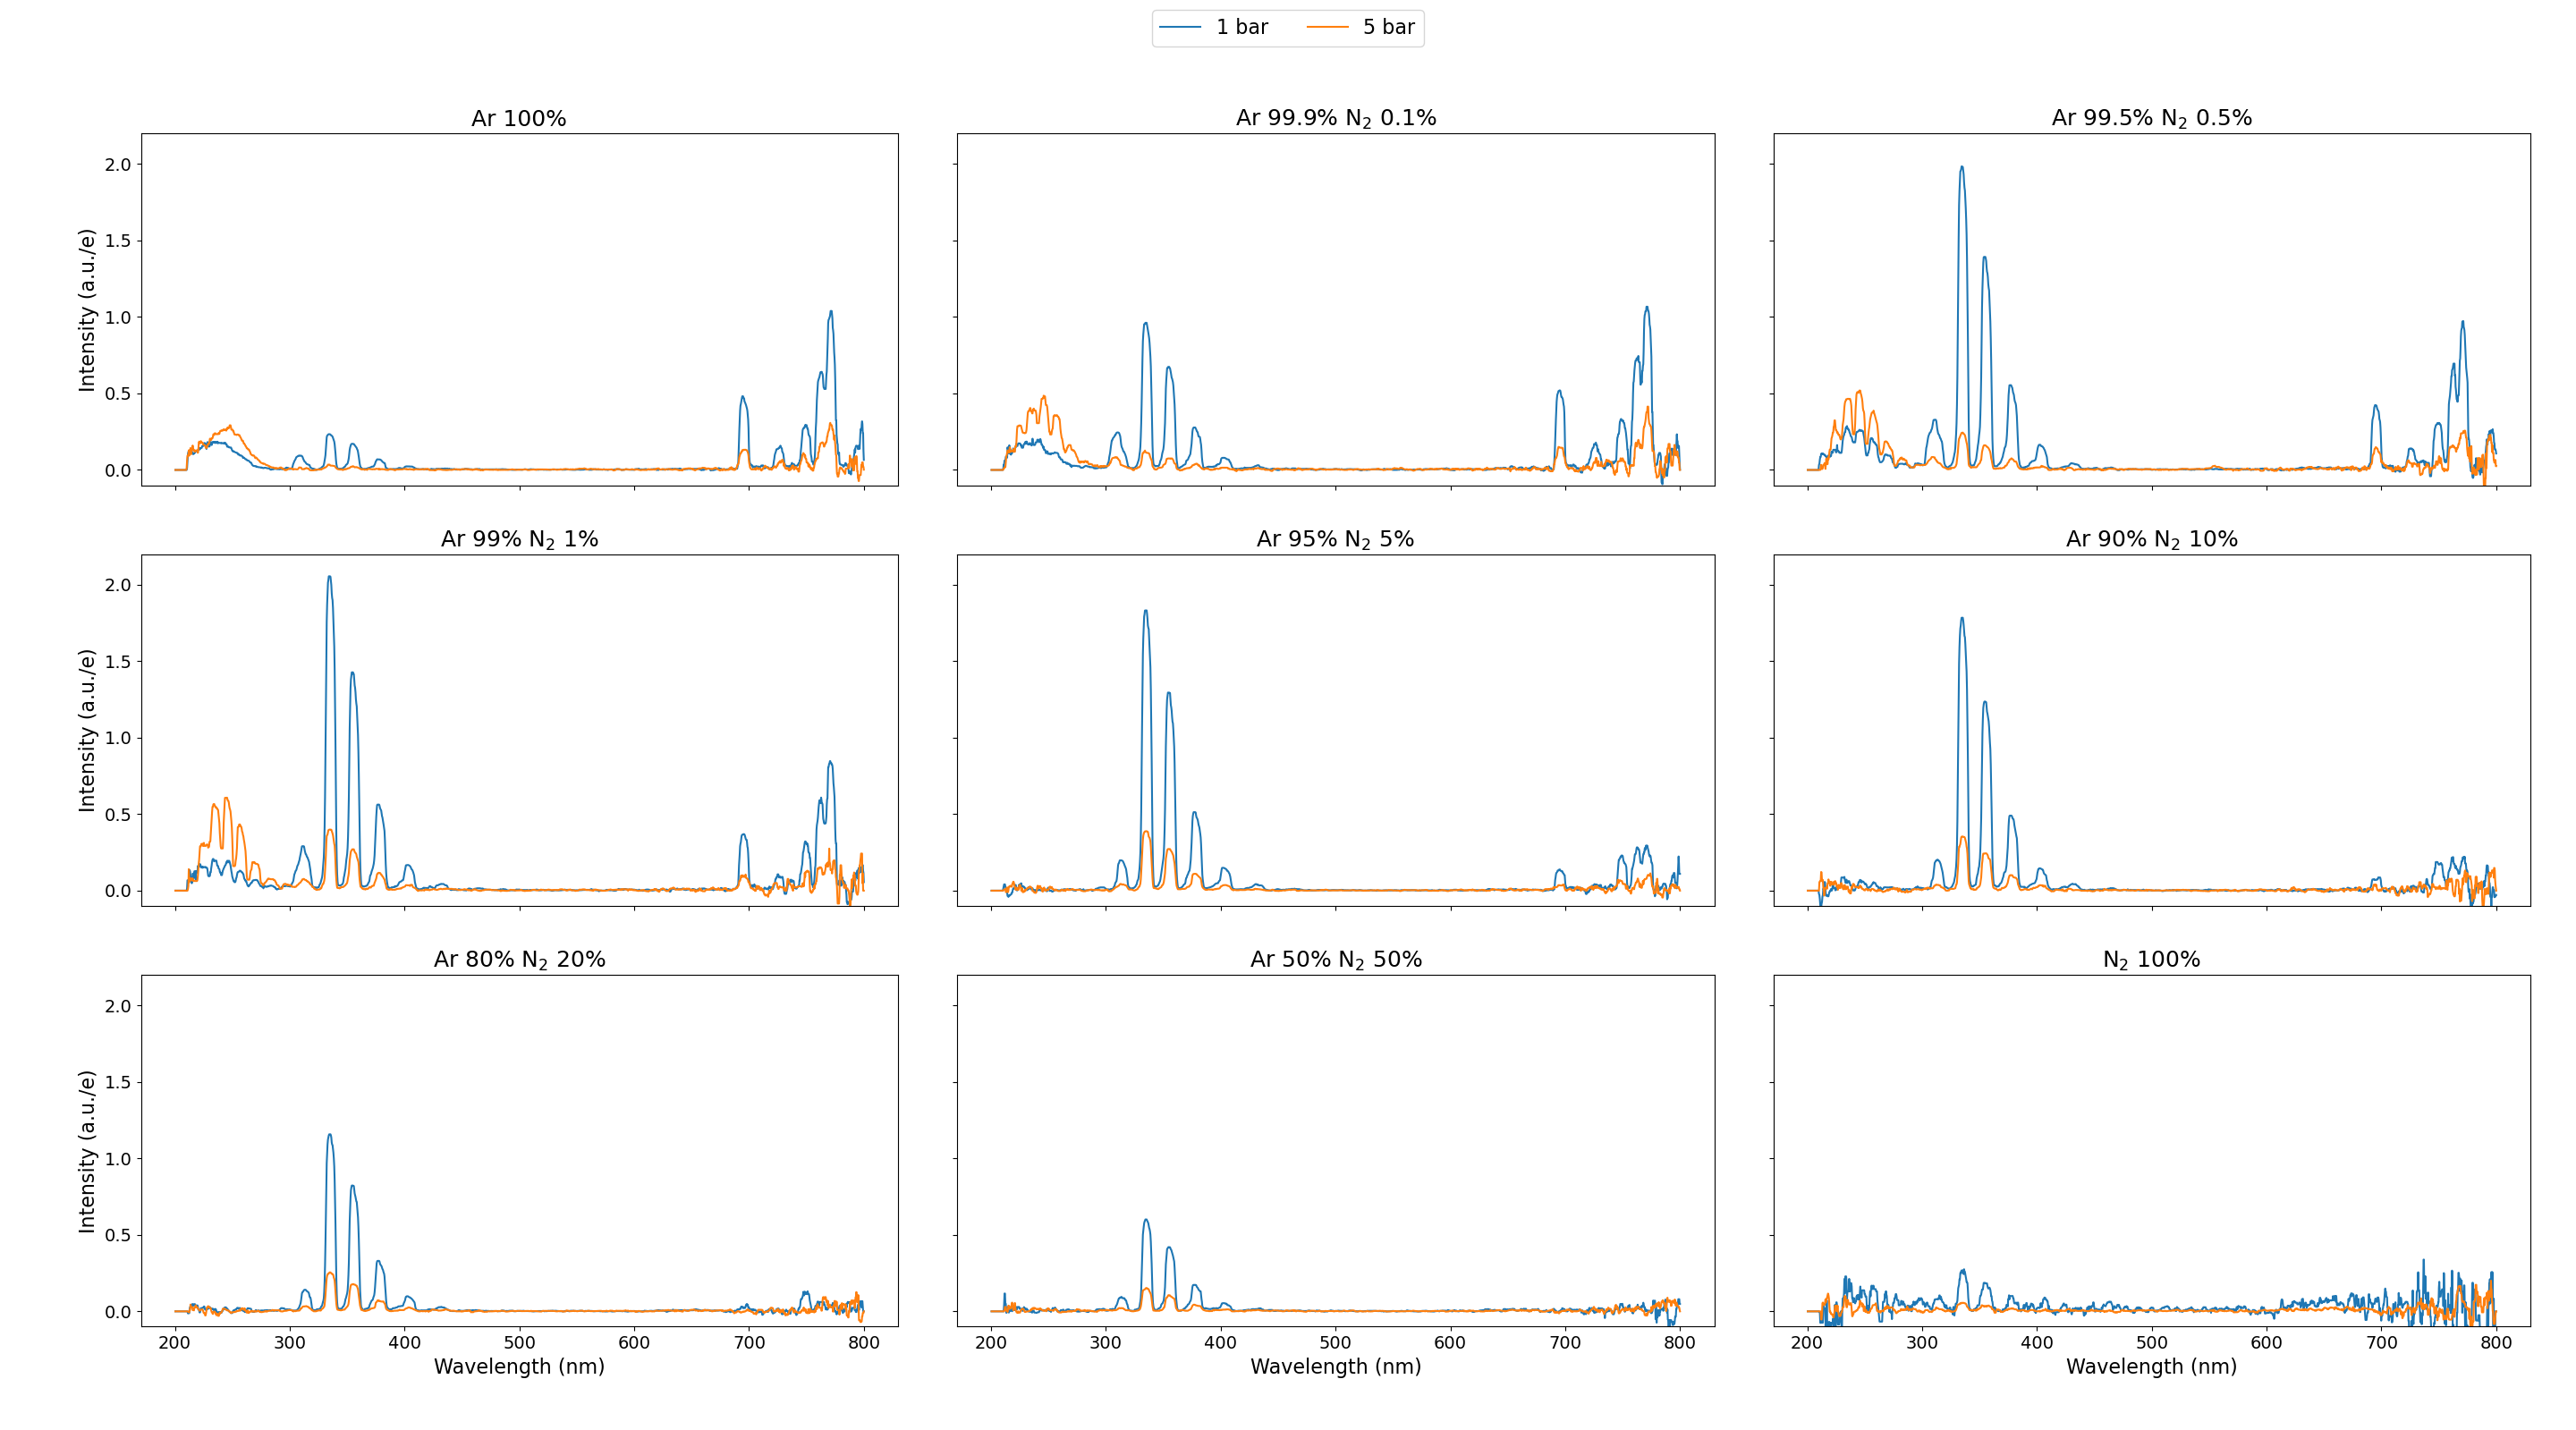
\includegraphics[width=0.95\linewidth]{experimental_espectra/Ar_N2_global_spectra.png}
    \caption{Espectro experimental global de la mezcla Ar--N$_2$. Datos de Raúl Señaris y Genaro Barco.}
    \label{fig:experimentalArN2GlobalEspectra}
\end{figure}

\section{Modelo Cinético} \label{Sec:model_kin}
% =================================================

\subsection{Introducción a los modelos cinéticos}


Los modelos cinéticos para la descripción de gases son herramientas análogas a los modelos radiativo-colisionales de la física de plasmas. Su objetivo es describir la evolución de las poblaciones de átomos, moléculas, iones y estados excitados cuando actúan simultáneamente procesos de producción, transferencia de energía, relajación colisional y emisión radiativa. En muchos problemas de centelleo no es necesario seguir la función de distribución completa de las partículas, sino que basta con describir la dinámica de las poblaciones de las especies relevantes mediante ecuaciones de balance.

Para una especie o estado excitado \(i\), la ecuación cinética general puede escribirse como
\begin{equation}
    \dv{N_i}{t}
    =
    S_i
    +
    \sum_j N_j R_{j\to i}
    -
    N_i \sum_k R_{i\to k},
    \label{eq:general_kinetic_balance}
\end{equation}
donde \(N_i\) es la población de la especie \(i\), \(S_i\) representa su producción directa, y los coeficientes \(R_{j\to i}\) y \(R_{i\to k}\) agrupan las tasas de formación y destrucción debidas a colisiones, transferencias de carga, disociaciones, relajaciones no radiativas o decaimientos radiativos.

En el caso de un estado excitado concreto, la destrucción suele venir dada por la competencia entre emisión espontánea y desexcitación colisional. Si el estado \(i\) posee una vida media radiativa \(\tau_i\) y puede ser desactivado por colisión con distintas especies \(m\), de densidad \(n_m\), con coeficientes cinéticos \(K_{iQ(m)}\), entonces la tasa total de desaparición del estado viene dada por
\begin{equation}
    \Gamma_i^{\text{tot}}
    =
    \frac{1}{\tau_i}
    +
    \sum_m n_m K_{iQ(m)}.
    \label{eq:total_loss_rate}
\end{equation}

Bajo condiciones estacionarias, \(\dv*{N_i}{t}=0\), la población del estado queda determinada por el cociente entre su tasa total de producción y su tasa total de pérdida:
\begin{equation}
    N_i
    =
    \frac{S_i + \sum_j N_j R_{j\to i}}
    {\Gamma_i^{\text{tot}}}.
    \label{eq:stationary_population}
\end{equation}

Más útil que la población absoluta es, en muchos casos, la probabilidad de que un estado excitado evolucione a través de un canal concreto. Si un proceso \(x\) compite con el resto de canales de desexcitación, su probabilidad viene dada por la razón entre su tasa parcial y la tasa total:
\begin{equation}
    P_{i\to x}
    =
    \frac{\Gamma_{i\to x}}
    {\Gamma_i^{\text{tot}}}.
    \label{eq:branching_ratio_general}
\end{equation}
De este modo, si el canal \(x\) corresponde a una colisión con una especie \(m\), se obtiene
\begin{equation}
    P_{i\to m}
    =
    \frac{n_m K_{iQ(m)}}
    {\dfrac{1}{\tau_i} + \sum_\ell n_\ell K_{iQ(\ell)}},
    \label{eq:branching_collision}
\end{equation}
mientras que si el canal considerado es radiativo,
\begin{equation}
    P_{i\to \gamma}
    =
    \frac{1/\tau_i}
    {\dfrac{1}{\tau_i} + \sum_\ell n_\ell K_{iQ(\ell)}}.
    \label{eq:branching_radiative}
\end{equation}

En una mezcla binaria genérica \(A-B\), con densidad total \(n\) y fracción molar \(f\) de \(A\), las densidades parciales vienen dadas por
\begin{equation}
    n_{A}=n\,f,
    \qquad
    n_{B}=n\,(1-f).
\end{equation}
Por tanto, las probabilidades de evolución de un estado excitado quedan fijadas por la competencia entre los canales de colisión con argón, los canales de colisión con nitrógeno y los decaimientos radiativos intrínsecos. Esta estructura conduce directamente a expresiones del tipo
\begin{equation}
    P
    =
    \frac{n\,f\,K_{\text{canal}}}
    {n\,f\,K_{\text{canal}}
    +
    n\,(1-f)\,K_{\text{competencia}}
    +
    1/\tau},
    \label{eq:generic_probability_binary_mixture}
\end{equation}
que son precisamente las que aparecen en el modelo cinético empleado para describir el centelleo en la mezcla $\Ar-\N_2$. La constante de Loschmidt 

$$ n_0 = \SI{2.6868e25}{m^{-3}} $$

nos da el número de moléculas que hay en un gas ideal a 1 atm y a 273.15 K. Así pues, si solo modificamos la presión siempre podemos expresar la densidad molar como:  

$$ n = (p/p_0) \cdot  n_0 $$

Nosotros incluiremos esta $n_0$ dentro de los coeficientes cinéticos $K$, que ahora tendrán unidades de ns$^{-1}$. Denotaremos a partir de ahora $n=p/p_0$ siendo $p_0 = \SI{1}{bar}$.

A partir de estas probabilidades de rama, el rendimiento de emisión asociado a una determinada banda espectral puede construirse como la suma de todas las vías de producción que alimentan la especie centelleadora, ponderadas por la probabilidad de que dicha especie se forme y, posteriormente, emita radiativamente antes de ser extinguida por colisión. 

\subsection{Ar--N$_2$} \label{subbsec:kinArN2}


\subsubsection{Procesos cinéticos}

Los decaimientos de estados del argón superiores (denotados por $\Ar^{**}$) que decaen siempre a alguno de las excitaciones resonante (1s5) y metaestable (1s4)

\begin{itemize}
    \item Decaimiento del $\Ar^{**}$ a $\Ar_{1s4,1s5}$
    \begin{equation}
        \Ar^{**} 
        \xrightarrow{\tau_{\Ar^{**}}}  \Ar_{1s4,1s5} + h \nu (\text{IR})
    \end{equation}
    \item Quenching con el nitrógeno
    \begin{equation}
        \Ar^{**} + \N_2
        \xrightarrow{K_{\Ar^{**}Q(\N_2)}}  \text{Estados no radiativos}
    \end{equation}
    \item Quenching con el argón
    \begin{equation}
        \Ar^{**} + \Ar
        \xrightarrow{K_{\Ar^{**}Q(\Ar)}}  \text{Estados no radiativos}
    \end{equation}
\end{itemize}


A partir de estos el argón resonante (1s5) y el metaestable (1s4) pueden tener las siguientes interacciones

\begin{itemize}
    \item Quenching del $\Ar_{1s4,1s5}$ con 2$\Ar$
    \begin{equation}
        \Ar_{1s4,1s5} + 2 \Ar
        \xrightarrow{K_{\Ar_{1s4,1s5,Q(2\Ar)}}}  \text{Estados no radiativos}
    \end{equation}

    \item Trasferencias del $\Ar_{1s4,1s5}$ con $N_2$ dando lugar a $N_2$ no radiativo.
    \begin{equation}
        \Ar_{1s4,1s5} + \N_2
        \xrightarrow{K_{\Ar_{1s4,1s5,Q(2\Ar)}}}  \Ar + N_2^{(*)}
    \end{equation}
    
    \item Trasferencias del $\Ar_{1s4,1s5}$ con $N_2$ dando lugar a $N_2(C)$
    \begin{equation}
        \Ar_{1s4,1s5} + \N_2
        \xrightarrow{K_{\Ar_{1s4,1s5,Q(N_2(C))}}}  \Ar + N_2^*(C)
    \end{equation}
\end{itemize}
Mientras que el $N_2$: 


\begin{itemize}
    \item Quenching del $\N_2(C)$ con $\Ar$
    \begin{equation}
        \N_2(C) +  \Ar
        \xrightarrow{K_{\N_2,Q(\Ar)}}  \text{Estados no radiativos}
    \end{equation}

    \item Quenching del $\N_2(C)$ con $\N_2$
    \begin{equation}
        \N_2(C) +  \N_2
        \xrightarrow{K_{\N_2,Q(\N_2)}}  \text{Estados no radiativos}
    \end{equation}

    \item Decaimiento del $\N_2(C)$
    \begin{equation}
        \N_2(C,v=0) \xrightarrow{\tau_{\N_2(C)}}  \N_2(B) + h\nu (330-410\mathrm{nm})
    \end{equation}
\end{itemize}

\hspace*{1em}\begin{table}[h!]
    \scriptsize
    \centering
    \begin{tabular}{lcccccc}
        \toprule
        {\bf Parameter} & \cite{friedl2012spectral} & \cite{puech1977energy} & \cite{buzulutskov2017photon} & \cite{zhang2018femtosecond} & \cite{Sauerbrey1981}  & Other \\
        
        \midrule
        
        $1/\tau_{\NC}$ [$\unit{s^{-1}}$]  & $\SI{2.6e7}{}$ & $\SI{2.07e7}{}$ & $\begin{matrix}
            \SI{3.3e7}{} \\
            \SI{2.5e7}{}
        \end{matrix}$ & $\SI{2.74e7}{}$ & $\SI{2.66e7}{}$ \\[1.5em]
        
        $k_{\NC Q(N_2^{*})}$ [$\unit{m^3 s^{-1}}$] &  $\SI{7.1e-18}{}$ & $\SI{1.12e-17}{}$ & $\SI{1e-17}{}$ & $\SI{1.4e-17}{}$ & $\SI{1e-18}{}$ \\[0.7em]
        
        $k_{\NC Q(\Ar)}$ [$\unit{m^3 s^{-1}}$] & - & $\SI{5.6e-19}{}$ & - & $\SI{8.6e-19}{}$ & $\SI{5.6e-19}{}$ \\[0.4em]
        
        \midrule
        
        $k_{\Ar^*(1s5) Q(\NC)}$ [$\unit{m^3 s^{-1}}$] & $\SI{3.2e-17}{}$ & $\SI{3.0e-17}{}$ & - & - & $\SI{1.1e-17}{}$ \\[0.7em] 
        $k_{\Ar^*(1s5) Q(\N_2)}$ [$\unit{m^3 s^{-1}}$] & - & - & - & - & $\SI{1.26e-17}{}$ \\[0.7em] 
        $k_{\Ar^*(1s5) Q(2\Ar)}$ [$\unit{m^6 s^{-1}}$] & -  & - &  - & - & $\SI{1e-44}{}$ & $\SI{7.93e6}{s^{-1}}$ \\[0.4em]
        
        \midrule
        
        $k_{\Ar^*(1s4) Q(\NC)}$ [$\unit{m^3 s^{-1}}$]  & - & $\SI{3.0e-17}{}$ & $\begin{matrix}
            \SI{1.5e-17}{} \\
            \SI{3.6e-17}{} 
        \end{matrix}$ & - & - \\[1.5em] 
        
        $k_{\Ar^*(1s4) Q(\N_2)}$ [$\unit{m^3 s^{-1}}$]  & - & - & $\begin{matrix}
            \SI{3e-17}{} \\
            \SI{3.6e-17}{} 
        \end{matrix}$ & - & - \\[1.5em] 
        
        $k_{\Ar^*(1s4) Q(2\Ar)}$  [$\unit{m^6 s^{-1}}$] & - & - &  $\SI{1e-44}{}$  & - & $\SI{1e-44}{}$ & $\SI{9.24e5}{s^{-1}}$  \\[0.7em]
        
        %\midrule
        %${\tau_{\Ar^{**}}}$  & - & - &  & - & -  \\[0.7em] 
        %$k_{\Ar^{**} Q(\N2)}$ & - & - & - & - & - \\[0.7em] 
        %$k_{\Ar^{**} Q(\Ar)}$ & - & - & - & - & -  \\[0.4em] 
        
        \bottomrule
    
    \end{tabular}
    \caption{Parameters in the literature}
    \label{tab:ArN2litearture}
\end{table}

\begin{figure}[h!]
    \centering
    
\includegraphics[width=0.5\linewidth]{kinetic_models/Kinetics_Models-1.pdf}
    \caption{Modelo cinético para Ar--N$_2$.}
    \label{fig:ArN2_kinetic_model}
\end{figure}

\subsubsection{Modelo cinético Ar--N$_2$} \label{subsubsec:modelkinArN2}

Así pues, el centelleo de una mezcla de $\Ar-\N_2$ viene dado por

\begin{equation}
    Y_{\N_2}
    =
    P_{\NC}
    \cdot
    \pqty{
      N_{\N_2^*}\cdot P_{\N_2}
      +
      N_{\ArOneSFour}\cdot P_{\ArOneSFour}
      +
      N_{\ArOneSFive}\cdot P_{\ArOneSFive} +
      N_{\Ar^{**}}\cdot P_{\Ar^{**}}
    }. \label{eq:YuvN2}
\end{equation} 

\begin{equation}
    P_{\NC}
    =
    \frac{1/\tau_{\NC}}{
    1/\tau_{\NC}
    +
    n \cdot f \cdot K_{\NC Q(\N_2)}
    +
    n \cdot (1-f) \cdot K_{\NC Q(\Ar)}}.
\end{equation}

\begin{equation}
    P_{\ArOneSFive}
    =
    \frac{n \cdot f \cdot K_{\ArOneSFive Q(\NC)}}{
    n \cdot f \cdot K_{\ArOneSFive Q(\NC)}
    +
    n^2 \cdot f \cdot K_{\ArOneSFive Q(2\Ar)}}.
\end{equation}

\begin{equation}
    P_{\ArOneSFour}
    =
    \frac{n \cdot f \cdot K_{\ArOneSFour Q(\NC)}}{
    n \cdot f \cdot K_{\ArOneSFour Q(\NC)}
    +
    n^2 \cdot f \cdot K_{\ArOneSFour Q(2\Ar)}}.
\end{equation} 
\begin{equation*}
    P_{\Ar^{**}}
    =
    \frac{\tau_{\Ar^{**}}}{\tau_{\Ar^{**}} + 
    n \cdot f \cdot K_{\ArOneSFour Q(\N_2)}
    +
    n \cdot (1-f) \cdot K_{\ArOneSFour Q(\Ar)}} \cdot (f_{\Ar^{**}} P_{\ArOneSFour} + (1-f_{\Ar^{**}}) P_{\ArOneSFive}) . 
\end{equation*}

La única constante efectiva que tendremos es $P_{\N_2}$, que contendrá la información acerca la fracción de estados de $\N_2^*$ que acaban en la banda vibracional $v=0$, estados  que emiten en las longitudes de onda de interés.

\subsection{Infrarrojo en Ar--N$_2$} \label{subbsec:kinArIR}

Los mecanismos de interacción que consideraremos son. 

\begin{minipage}{0.55\linewidth} 
\begin{itemize}
    \item Decaimiento de la especie: 
    
    \begin{equation}
        \Ar^*_\lambda \xrightarrow{\tau_{\Ar^*_\lambda}}  \Ar + h\nu (\lambda 
  \ \mathrm{nm})
    \end{equation}
    
    \item Quenching con argón:

    \begin{equation}
        \Ar^*_\lambda +  \Ar
        \xrightarrow{K_{\Ar^*_\lambda,Q(\Ar)}}  \text{Estados no radiativos}
    \end{equation}
    
    \item Quenching con un aditivo molecular $(\N_2)$: 

    \begin{equation}
        \Ar^*_\lambda + X       \xrightarrow{K_{\Ar^*_\lambda,Q(\N_2)}}  \text{Estados no radiativos}
    \end{equation}
    
\end{itemize}
\end{minipage} \hfill
\begin{minipage}{0.42\linewidth} \centering
    
\includegraphics[width=0.96\linewidth]{kinetic_models/Kinetics_Models-4.pdf}
    \captionof{figure}{Modelo cinético Ar IR.} \label{fig:Ar_IR_kinetic_model}
\end{minipage}


Las emisiones del infrarrojo del Ar se producen por especies muy concretas (apartado \ref{subsec:Ar_spectra}). Estas especies no pueden producirse por mecanismos de trasferencia por parte de otras especies de argón o del aditivo molecular, por lo que solo debemos considerar la producción directa de los mismos. No obstante, si pueden producirse por el decaimiento de excitaciones más energéticas. Entonces $ N_{\Ar^*,\lambda}$ será la suma todos las excitaciones más energéticas que la que emite, y $P_{\Ar^*,\lambda}$ será el producto de la fracción de estados realmente involucrados y la probabilidad de que estos lleven a la especie centelladora. Una vez llegan a esta entra la competencia entre decaimiento y fenómenos de quenching (véase figura \ref{fig:Ar_IR_kinetic_model}). Así el modelo cinético de la emisión infrarroja para el pico de longitud de onda $\lambda$

\begin{equation}
    Y_{\mathrm{IR},\lambda} = P_{\Ar^*,\lambda} \cdot N_{\Ar^*,\lambda}  \cdot \pqty{\frac{1 / \tau_{\Ar^*,\lambda}}{1 / \tau_{\Ar^*,\lambda} + n \cdot f \cdot  K_{\Ar^*, Q(\Ar), \lambda} + n \cdot(1-f) \cdot  K_{\Ar^*, Q(\N_2), \lambda}} }
\end{equation}

\section{Simulaciones} 
% =================================================

Para obtener la población media de cada estado por evento, \(N_X\), se han utilizado dos herramientas complementarias: Degrad para la descripción de la interacción primaria, y Garfield++ la descripción del centelleo secundario. Esta combinación permite separar de forma natural dos escalas físicas distintas. Por un lado, la creación del primario depende del tipo de partícula incidente y de sus mecanismos de ionización inicial. Por otro, el desarrollo de la avalancha, la producción de excitaciones y la creación de electrones secundarios están dominados por el campo eléctrico local y por las secciones eficaces electrón--átomo/molécula de la mezcla. 

Desde el punto de vista cinético, la magnitud de entrada fundamental son las secciones eficaces \(\sigma_j(\varepsilon)\) asociadas a cada canal microscópico \(j\) (colisión elástica, excitación, ionización, attachment, \emph{etc.}), donde \(\varepsilon\) es la energía cinética del electrón. En términos prácticos, esto implica que las poblaciones \(N_X\) por evento pueden interpretarse como el resultado acumulado de todas las colisiones de excitación, ionización o attachment sufridas por el electrón primario y por todos sus descendientes a lo largo de la avalancha.


Dado que en ambos casos se utiliza un conjunto consistente de secciones eficaces, las poblaciones obtenidas con Degrad y Garfield++ son comparables aunque correspondan a fenómenos distintos. En las figuras~\ref{fig:ArCs} y \ref{fig:N2Cs} se muestran las secciones eficaces empleadas para $\Ar$ y $\N_2$, distinguiendo canales elásticos, de ionización e inelásticos/excitadores.

\begin{minipage}{0.5\linewidth}
    \centering
    
\includegraphics[width=0.99\linewidth]{cross_sections/Ar_cs.pdf}
    \captionof{figure}{Secciones eficaces del argón.}
    \label{fig:ArCs}
\end{minipage} \hfill
\begin{minipage}{0.5\linewidth}
    \centering
    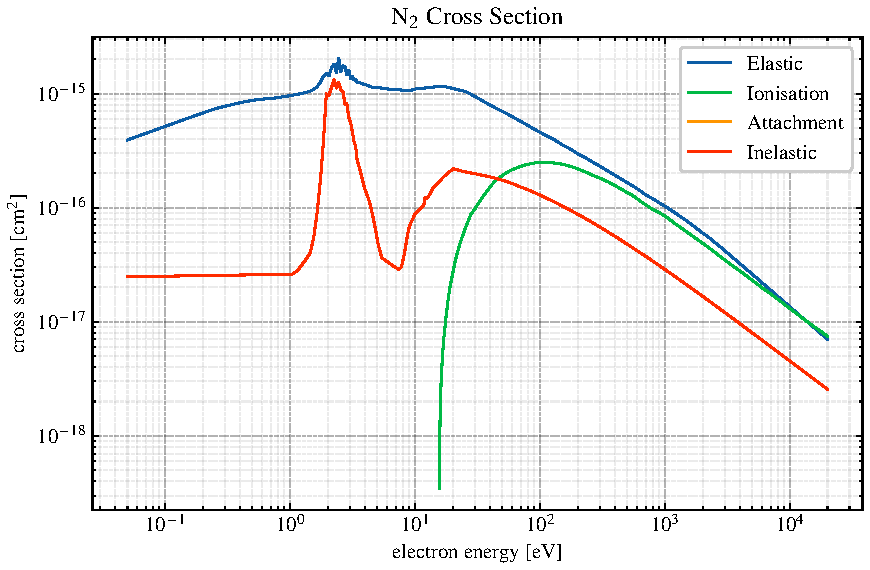
\includegraphics[width=0.70\linewidth]{cross_sections/N2_cs.pdf}
    \captionof{figure}{Secciones eficaces del $\N_2$.}
    \label{fig:N2Cs}
\end{minipage}

\subsection{Garfield++}

{Garfield++} es un entorno en \texttt{C++} orientado a la simulación detallada de detectores gaseosos y semiconductores basados en ionización. En el contexto de gases, su interés principal reside en la posibilidad de realizar seguimiento microscópico electrón por electrón, colisión por colisión, utilizando para ello las tasas de interacción tabuladas por {Magboltz}. Dado que {Magboltz}, también desarrollado por Steve Biagi, calcula propiedades de transporte y tasas de colisión a partir de secciones eficaces microscópicas, la combinación {Garfield++} y {Magboltz} permite pasar de la microfísica de dispersión a observables macroscópicos como deriva, difusión, coeficiente de Townsend, attachment, ganancia y producción de estados excitados.

En este trabajo, Garfield++ se emplea en modo de seguimiento microscópico de los electrones. En este esquema, el electrón se propaga entre colisiones siguiendo una trayectoria clásica determinada por el campo eléctrico local. La duración del vuelo libre se muestrea a partir de la frecuencia total de colisión, y el tipo de interacción que tiene lugar al final del paso se selecciona de acuerdo con las tasas relativas de cada proceso. Este procedimiento es especialmente adecuado para mezclas con canales competitivos muy distintos entre sí, como ocurre en $\Ar-\N_2$, donde coexisten excitación, ionización y pérdidas inelásticas con umbrales energéticos diferentes, donde coexisten excitación, ionización, attachment y pérdidas inelásticas con umbrales energéticos diferentes. Gaffield++ tiene la capacidad de escalar a altras energías las ele

El algoritmo utilizado por {Garfield++} para el muestreo del tiempo de vuelo es el método de Monte Carlo con colisiones nulas (\textit{null-collision Monte Carlo}, también conocido como MCC o técnica NC). La idea básica consiste en introducir una frecuencia ficticia adicional que permita muestrear los vuelos libres con una tasa mayorante simple; cuando el proceso sorteado corresponde a una ``colisión nula'', la partícula no cambia de estado físico y simplemente continúa su movimiento. Aunque estas colisiones virtuales no tienen significado físico directo, el método reproduce correctamente la estadística de los procesos reales y resulta muy eficiente cuando las tasas de colisión dependen fuertemente de la energía del electrón. De hecho, en {Garfield++} las colisiones virtuales aparecen explícitamente en la clasificación interna de procesos como \textit{virtual (null) collisions}.

\subsection{Aproximación de campo uniforme y desarrollo de la avalancha}

Para la simulación de la multiplicación secundaria se ha adoptado la geometría de deriva uniforme mostrada en la Fig.~\ref{fig:uniformDrift}. Esta aproximación consiste en suponer que, en la región efectiva donde se desarrolla la avalancha, el campo eléctrico es aproximadamente constante:
\begin{equation}
    \mathbf{E}(\mathbf{r}) \simeq E_0\, \hat{\mathbf{z}}.
\end{equation}
La hipótesis es razonable cuando el hueco de amplificación es pequeño y el objetivo principal es estimar la estadística de colisiones, la ganancia y la producción media de excitaciones, en lugar de resolver con máximo detalle las no uniformidades locales de la geometría real. Bajo esta aproximación, las diferencias entre electrones vienen dadas sobre todo por la secuencia aleatoria de colisiones, y no por variaciones geométricas del campo.

La avalancha electrónica se construye entonces de manera jerárquica. El electrón primario, introducido directamente en {Garfield++}, atraviesa la región de deriva y, si su energía entre colisiones supera los umbrales relevantes, puede producir excitaciones o ionizaciones. Cada colisión de ionización genera un nuevo electrón secundario que, a su vez, es transportado microscópicamente por el mismo algoritmo y puede originar ionizaciones adicionales. El resultado final es una cascada ramificada, tal y como podemos ver en la figura \ref{fig:uniformDrift} en la que el primario y todos sus descendientes contribuyen a la ganancia total y a las poblaciones \(N_X\) de las distintas especies excitadas. En la figura \ref{fig:gainNe} podemos ver un histograma donde vemos el número de electrones genreados por electrón primario simulado (electrón inicial). A este número se le llama ganancia electrónica (o de carga) y se la denota como $n_e$. 

Desde el punto de vista del modelo cinético, esta cascada puede resumirse como una suma sobre trayectorias electrónicas. Si \(N_X^{(k)}\) es el número de veces que el proceso \(X\) aparece en la historia del electrón \(k\), el número total por evento viene dado por
\begin{equation}
    N_X = \sum_{k \ \in \ \mathrm{avalancha}} N_X^{(k)}.
    \label{eq:NX_event}
\end{equation}
Equivalentemente, en promedio, \(N_X\) queda determinado por la integral de las probabilidades de colisión a lo largo de todas las trayectorias del primario y de los secundarios. Esta es precisamente la magnitud que después se introduce en el modelo cinético-radiativo para estimar los distintos canales de emisión de la mezcla.




\begin{figure}[h!]
    \centering
    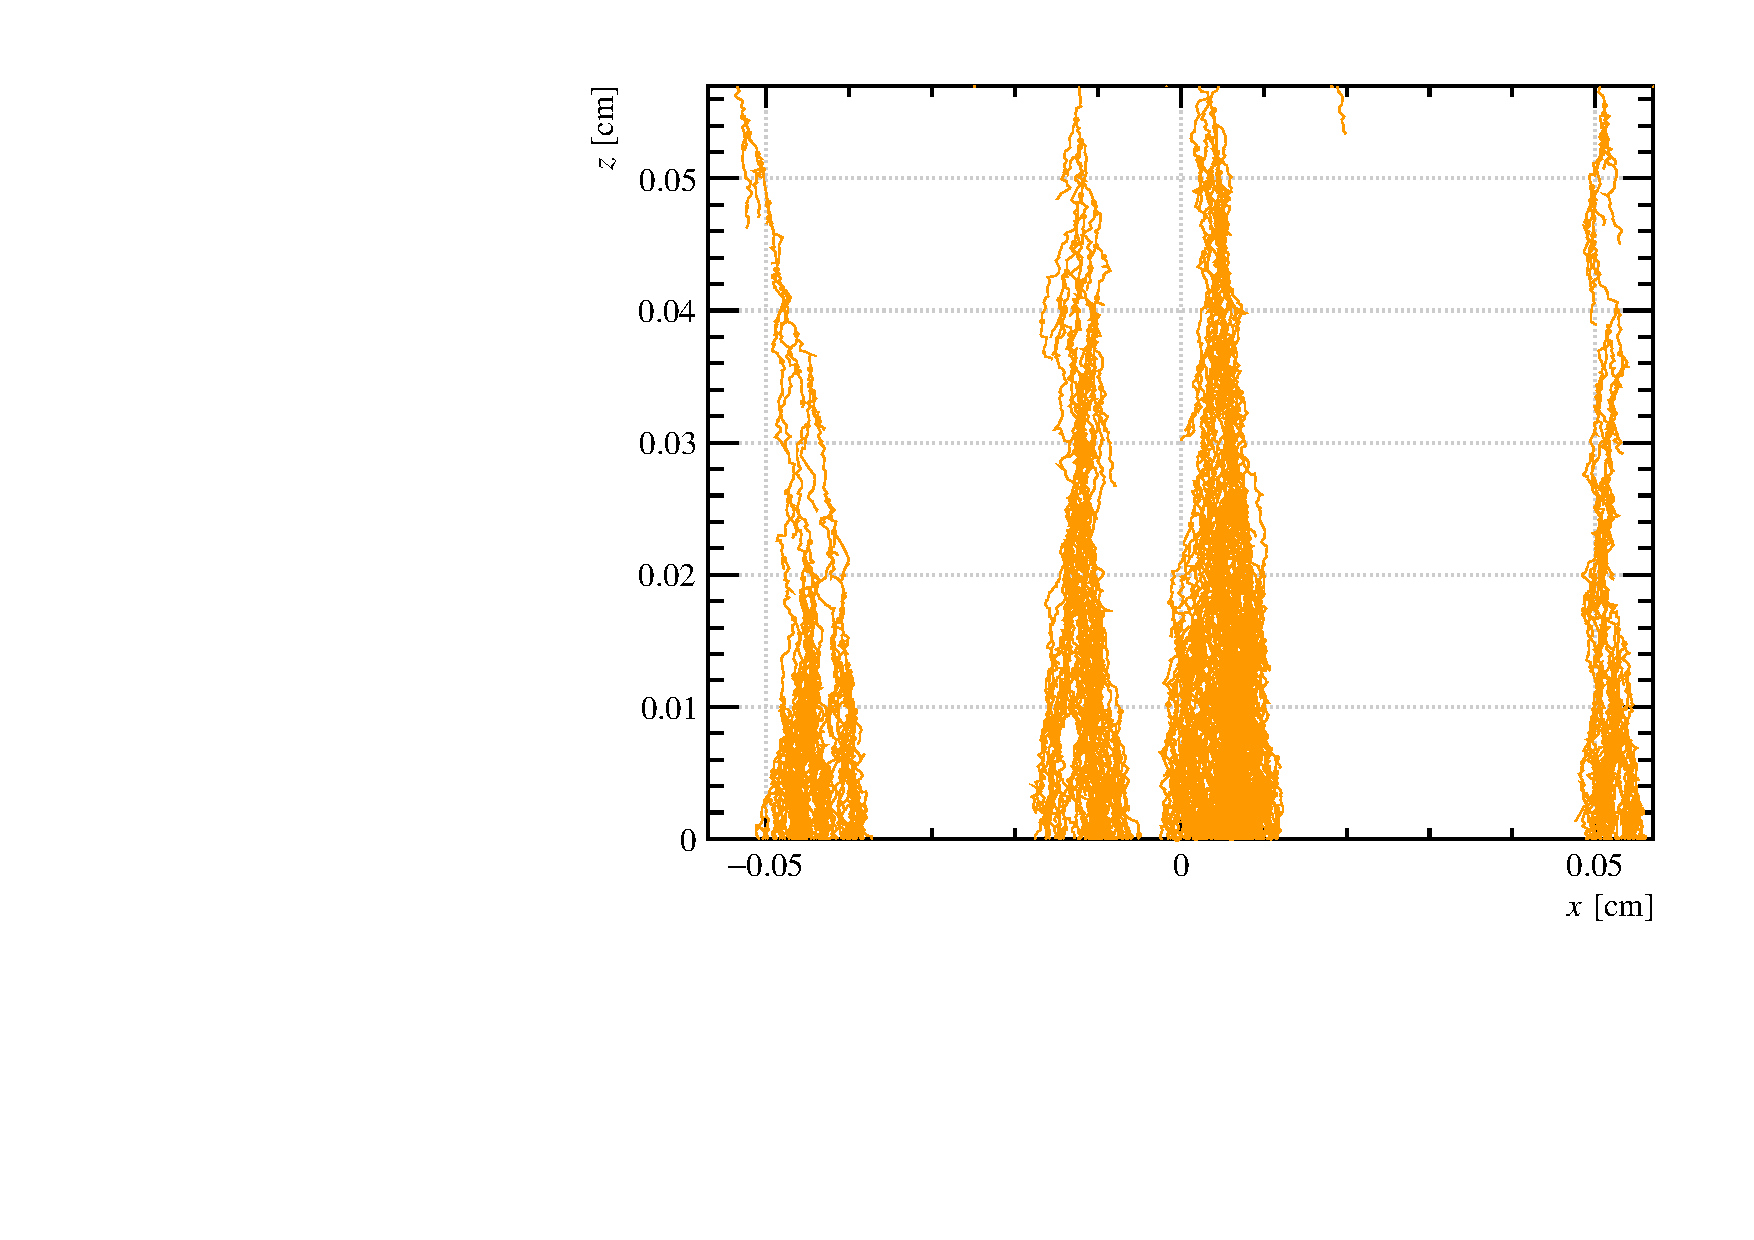
\includegraphics[width=0.46\linewidth]{garfield++/uniform_drift.pdf}
    \caption{Esquema de la cascada electrónica en la aproximación de campo uniforme.}
    \label{fig:uniformDrift}
\end{figure}


% =================================================
\section{Obtención de Parámetros}
% =================================================

En Ar--N$_2$ existen coeficientes cinéticos publicados para varios procesos de transferencia y \emph{quenching}, aunque sus valores muestran dispersión entre medidas. En este trabajo dichos coeficientes se toman como referencias semi-restringidas dentro del ajuste, permitiendo variaciones alrededor de sus valores nominales, mientras que las probabilidades efectivas describen la fracción de estados simulados que termina alimentando la banda radiativa observada.

La comparación entre poblaciones simuladas y rendimientos experimentales requiere incluir un factor de normalización común $N_{\norma}$ y el potencial medio de ionización de la mezcla. Para una fracción molar $f_{\N_2}$ se emplea
\begin{equation}
    W_I(f_{\N_2}) = \frac{1}{f_{\N_2}/W_{\N_2} + (1-f_{\N_2})/W_{\Ar}}.
\end{equation}
El ajuste de la emisión UV se realiza sobre la segunda banda positiva del nitrógeno, integrando las contribuciones de producción directa y de transferencia energética desde estados excitados del argón.

\subsection{Tratamiento de errores sistemáticos y estadísticos}

Los datos experimentales empleados en el ajuste presentan, en general, dos contribuciones principales a la incertidumbre: una componente estadística y una componente sistemática. Ambas tienen un origen físico y experimental distinto, por lo que no deben tratarse de la misma manera. Las incertidumbres estadísticas describen fluctuaciones aleatorias independientes asociadas, por ejemplo, al número finito de eventos, a la dispersión de las medidas o al proceso de extracción de los puntos experimentales. En cambio, las incertidumbres sistemáticas suelen estar asociadas a efectos comunes de calibración, eficiencia óptica, normalización, respuesta espectral o escala absoluta de intensidad. Por tanto, mientras que la componente estadística puede considerarse, en primera aproximación, independiente punto a punto, la componente sistemática debe tratarse como una fuente de desplazamiento correlacionado entre varios puntos de un mismo conjunto de datos. Esta distinción es habitual en el análisis estadístico de experimentos de física de partículas, donde las incertidumbres sistemáticas se introducen mediante parámetros auxiliares o \textit{nuisance parameters} gaussianamente constreñidos \cite{Barlow2002,Cowan2011,Conway2011,Cranmer2012HistFactory,PDGStatistics2024}.

En este trabajo, el ajuste nominal se realiza empleando las incertidumbres estadísticas de los datos experimentales. Dado un modelo $f(x;\boldsymbol{\theta})$, donde $\boldsymbol{\theta}$ representa el vector de parámetros libres, los parámetros óptimos $\hat{\boldsymbol{\theta}}$ se obtienen minimizando la suma de residuos ponderados,

\[
r_i(\boldsymbol{\theta})=
\frac{y_i-f(x_i;\boldsymbol{\theta})}
{\sigma_{i,\mathrm{stat}}},
\]

mediante la rutina \texttt{least\_squares} de \texttt{scipy.optimize} \cite{Virtanen2020SciPy}. Esta elección define la curva central del modelo, que se interpreta como la mejor descripción de los datos bajo las hipótesis físicas incorporadas al modelo. El uso exclusivo de la incertidumbre estadística en la función objetivo evita que las componentes sistemáticas, que no representan fluctuaciones independientes, sean tratadas como ruido aleatorio punto a punto. En particular, incluir directamente las incertidumbres sistemáticas en cuadratura dentro de cada residuo produciría un ajuste menos sensible a la estructura de los datos y, además, ignoraría las correlaciones entre puntos inducidas por una misma fuente sistemática.

Para propagar las incertidumbres a los parámetros y a las predicciones del modelo, se emplea un procedimiento basado en pseudoexperimentos. Este método resulta especialmente adecuado en el presente caso, ya que el modelo es no lineal y presenta degeneraciones importantes entre algunos parámetros. En estas condiciones, la estimación local de la matriz de covarianzas a partir del jacobiano del ajuste,

\[
\mathrm{Cov}(\hat{\boldsymbol{\theta}})
\simeq
s^2(J^TJ)^{-1},
\]

puede ser numéricamente inestable o difícil de interpretar. En particular, parámetros individuales pueden tener incertidumbres muy grandes debido a correlaciones internas del modelo, aunque la predicción física final permanezca relativamente bien determinada. Por este motivo, se prefiere propagar las incertidumbres directamente mediante réplicas fluctuadas de los datos y refitear el modelo en cada una de ellas. Este procedimiento es equivalente, en la práctica, a una propagación Monte Carlo de las incertidumbres experimentales y evita depender únicamente de una aproximación lineal alrededor del mínimo.

Para la componente estadística se generan pseudoexperimentos fluctuando cada punto de forma independiente,

\[
y_i^{(t)}
= 
y_i
+
\epsilon_i^{(t)},
\qquad
\epsilon_i^{(t)}
\sim
\mathcal{N}(0,\sigma_{i,\mathrm{stat}}),
\]

donde $t$ identifica la réplica generada. Cada conjunto fluctuado se ajusta de nuevo con el mismo modelo, obteniendo un vector de parámetros $\boldsymbol{\theta}^{(t)}$ y una predicción asociada $f(x;\boldsymbol{\theta}^{(t)})$. La distribución de estas predicciones proporciona una estimación directa de la incertidumbre estadística de la curva ajustada. En las figuras, la banda estadística se define mediante los percentiles 16 y 84 de las curvas obtenidas, que corresponden aproximadamente a una banda de una desviación típica para distribuciones gaussianas.

La componente sistemática se trata de forma diferente, ya que no representa fluctuaciones independientes de cada punto. Para ello se introducen variables gaussianas comunes, o \textit{nuisance parameters}, asociadas a cada fuente sistemática relevante. Si $\Delta_i^{(k)}$ representa el desplazamiento sistemático del punto $i$ debido a la fuente $k$, un pseudoexperimento sistemático se construye como

\[
y_i^{(t)}
=
y_i
+
\sum_k z_k^{(t)}\Delta_i^{(k)},
\qquad
z_k^{(t)}
\sim
\mathcal{N}(0,1).
\]

De este modo, todos los puntos afectados por una misma fuente sistemática se desplazan de forma coherente. En los datos UV de Ar--N$_2$ puede emplearse una fuente sistemática común para el conjunto correspondiente, mientras que en el infrarrojo resulta natural asignar una fuente sistemática a cada longitud de onda. Este tratamiento refleja mejor el significado físico de una incertidumbre sistemática: una calibración óptica o una eficiencia espectral no desplaza cada punto al azar, sino que modifica de manera correlacionada una familia completa de medidas.

Desde el punto de vista formal, este procedimiento es equivalente a construir una matriz de covarianza total con una parte estadística diagonal y una parte sistemática correlacionada,

\[
V
=
V_{\mathrm{stat}}
+
V_{\mathrm{syst}},
\]

donde

\[
V_{\mathrm{stat},ij}
=
\sigma_{i,\mathrm{stat}}^2\delta_{ij},
\]
y
\[
V_{\mathrm{syst},ij}
=\sum_k
\Delta_i^{(k)}\Delta_j^{(k)}.
\]

Esta forma de escribir la matriz de covarianza muestra explícitamente que una fuente sistemática común genera correlaciones entre distintos puntos experimentales. El enfoque mediante pseudoexperimentos evita tener que construir e invertir explícitamente esta matriz en cada ajuste, pero conserva la interpretación física de las correlaciones sistemáticas. Es, por tanto, una versión sencilla y transparente del tratamiento mediante parámetros auxiliares usado de forma estándar en análisis de altas energías, como en los métodos de \textit{profile likelihood} e implementaciones tipo \textsc{HistFactory} \cite{Cowan2011,Cranmer2012HistFactory}.

Finalmente, las incertidumbres de los parámetros se obtienen a partir de la dispersión de los valores ajustados en los distintos pseudoexperimentos. Para cada parámetro se calculan por separado una contribución estadística, procedente de las réplicas con fluctuaciones independientes punto a punto, y una contribución sistemática, procedente de las réplicas con desplazamientos correlacionados. Las predicciones finales del modelo para rendimientos primarios en $\mathrm{ph/MeV}$ se acompañan de bandas construidas a partir de los percentiles de las curvas refiteadas. Este tratamiento permite separar de manera clara la estabilidad estadística del ajuste y la sensibilidad a fuentes sistemáticas comunes, manteniendo al mismo tiempo una interpretación física coherente de ambas contribuciones. En los casos donde algunos parámetros presentan incertidumbres relativas grandes, estas deben interpretarse con cautela, ya que pueden reflejar degeneraciones internas del modelo más que una pérdida equivalente de precisión en la predicción final. Por ello, en este trabajo se da especial importancia a las bandas de predicción del modelo, que constituyen una estimación más robusta de la incertidumbre sobre las magnitudes físicamente observables.


\subsection{Ajuste UV de Ar--N$_2$}

Las ecuaciones para Ar--N$_2$ (recordando que $n=p/p_0$ siendo $p$ la presión y $p_0=1$ bar y $f$ es concentración del aditivo $\N_2$), realizadas a partir de las ecuaciones (\ref{eq:YuvN2}) son: 


\begin{equation*}
    \frac{Y_{\N_2}}{W_I(f)} 
    =
    {N_{\norma}}
    \cdot
    P_{\NC}
    \cdot
    \pqty{
      N_{\N_2^*}\cdot P_{\N_2}
      +
      N_{\ArOneSFour}\cdot P_{\ArOneSFour}
      +
      N_{\ArOneSFive}\cdot P_{\ArOneSFive}
      + N_{\Ar^{**}} \cdot P_{\Ar^{**}}
    }
\end{equation*}

\begin{equation}
    P_{\NC}
    =
    \frac{1/\tau_{\NC}}{
    1/\tau_{\NC}
    +
    n \cdot f \cdot K_{\NC Q(\N_2)}
    +
    n \cdot (1-f) \cdot K_{\NC Q(\Ar)}}
\end{equation}

\begin{equation}
    P_{\ArOneSFive}
    =
    \frac{n \cdot f \cdot K_{\ArOneSFive Q(\NC)}}{
    n \cdot f \cdot K_{\ArOneSFive Q(\NC)}
    +
    n^2 \cdot f \cdot K_{\ArOneSFive Q(2\Ar)}}
\end{equation}

\begin{equation}
    P_{\ArOneSFour}
    =
    \frac{n \cdot f \cdot K_{\ArOneSFour Q(\NC)}}{
    n \cdot f \cdot K_{\ArOneSFour Q(\NC)}
    +
    n^2 \cdot f \cdot K_{\ArOneSFour Q(2\Ar)}}
\end{equation}


\begin{equation*}
    P_{\Ar^{**}}
    = P_{\Ar^{**}}^* \cdot 
    \frac{\tau_{\Ar^{**}}}{\tau_{\Ar^{**}} + 
    n \cdot f \cdot K_{\ArOneSFour Q(\N_2)}
    +
    n \cdot (1-f) \cdot K_{\ArOneSFour Q(\Ar)}} \cdot (f_{\Ar^{**}} P_{\ArOneSFour} + (1-f_{\Ar^{**}}) P_{\ArOneSFive}) . 
\end{equation*}


Los resultados experimentales cuentan con 5 presiones (1, 2, 3, 4 y 5 bar) y 8 concentraciones diferentes (desde 0.1\% a 100\% $\N_2$), contamos con hasta 40 datos experimentales, lo que permite constreñir el modelo. Además usamos los valores de la literatura (tabla \ref{tab:ArN2litearture}) dejando variar únicamente un factor 2 sobre el valor de referencia. Dado que $P_{\Ar^{**}}^*$ y $P_{\N_2}^*$ están completamente correlacionados con $N_{\norma}$, no es posible desambiguar los tres valores únicamente con este conjunto de datos. Por ello se fija $N_{\norma}$ a partir de la calibración externa común empleada en la adquisición experimental. Además constreñimos $P_{\N_2}$ a un valor máximo de 0.7, que es la fracción de estados con $\N_2(C,v=0)$ respecto $\N_2(C,v=1,2,3)$ máxima hallada en el rango 0 - 1 bar de estados $v=0$ en la colaboración MACFLY \cite{colin2007macfly}. No incluimos un valor mínimo al poder haber más efectos además de la fracción de estados $v=0$.

En las gráficas \ref{fig:ArN2Fit} podemos ver el ajuste para el ajute con un factor 3. El ajuste obtenido con una $\chi^2_{\mathrm{red}}=0.4$ muestra que nuestro modelo es compatible con los datos. Además enseñamos en las figuras \ref{fig:ArN2Fit1bar} y \ref{fig:ArN2Fit5bar} las predicciones con las componentes desambiguadas, donde podemos ver claramente la diferencia en la forma funcional y la diferencia en el comportamiento con la presión entre el resonante (1s4) y el metaestable (1s5), debido a la diferencia entre los parámetros cinéticos. 

\begin{table}[htbp]
\centering
\caption{Parámetros del ajuste primario UV en Ar--N$_2$.}
\label{tab:ArN2_UV_toy_uncertainties}
\begin{tabular}{lccc}
\toprule
Parámetro & Valor & Estadístico & Sistemático \\
\midrule
$N_{\mathrm{norm}}$ & \num{4.46e-3} & -- & -- \\
$P_{\mathrm{N}_2}$ & \num{7e-1} & $^{+\num{0}}_{-\num{3.1e-14}}$ & $^{+\num{0}}_{-\num{4e-12}}$ \\
$\tau_{\mathrm{N}_2}$ & \num{3.78e1} & -- & -- \\
$K_{\mathrm{N}_2,Q(\mathrm{N}_2)}$ & \num{1.44e-1} & $^{+\num{2.7e-2}}_{-\num{1.5e-2}}$ & $^{+\num{1.4e-3}}_{-\num{2.3e-3}}$ \\
$K_{\mathrm{N}_2,Q(\mathrm{Ar})}$ & \num{3.48e-2} & $^{+\num{9e-17}}_{-\num{5.8e-3}}$ & $^{+\num{9e-17}}_{-\num{3.3e-13}}$ \\
$K_{\mathrm{Ar(1s4)},Q(\mathrm{N}_2,c)}$ & \num{8.44e-1} & $^{+\num{3.5e-1}}_{-\num{5.5e-1}}$ & $^{+\num{2e-1}}_{-\num{1.2e-3}}$ \\
$K_{\mathrm{Ar(1s4)},Q(\mathrm{N}_2,b)}$ & \num{1.96e-2} & $^{+\num{3.6e-12}}_{-\num{3.5e-18}}$ & $^{+\num{9.7e-14}}_{-\num{3.5e-18}}$ \\
$K_{\mathrm{Ar(1s4)},Q(2\mathrm{Ar})}$ & \num{1.59e-2} & $^{+\num{1e-14}}_{-\num{8.7e-3}}$ & $^{+\num{8.4e-15}}_{-\num{1.5e-12}}$ \\
$K_{\mathrm{Ar(1s5)},Q(\mathrm{N}_2,c)}$ & \num{1.25e0} & $^{+\num{8.4e-15}}_{-\num{4.1e-10}}$ & $^{+\num{8.4e-15}}_{-\num{2.7e-12}}$ \\
$K_{\mathrm{Ar(1s5)},Q(\mathrm{N}_2,b)}$ & \num{9.18e-2} & $^{+\num{1.1e-10}}_{-\num{1.4e-17}}$ & $^{+\num{8.6e-15}}_{-\num{1.4e-17}}$ \\
$K_{\mathrm{Ar(1s5)},Q(2\mathrm{Ar})}$ & \num{7.89e-4} & $^{+\num{2.4e-4}}_{-\num{3.3e-4}}$ & $^{+\num{8.2e-6}}_{-\num{6.7e-5}}$ \\
$P_{\mathrm{Ar}^{**}}^* $ & \num{2.27e-1} & $^{+\num{6.8e-2}}_{-\num{3.9e-2}}$ & $^{+\num{4.1e-2}}_{-\num{4.6e-2}}$ \\
$f_{\mathrm{Ar}^{**}}$ & \num{3.17e-1} & $^{+\num{3.8e-1}}_{-\num{1.3e-1}}$ & $^{+\num{7.3e-2}}_{-\num{1.3e-3}}$ \\
\bottomrule
\end{tabular}
\end{table}

\begin{figure}[h!]
    \centering
    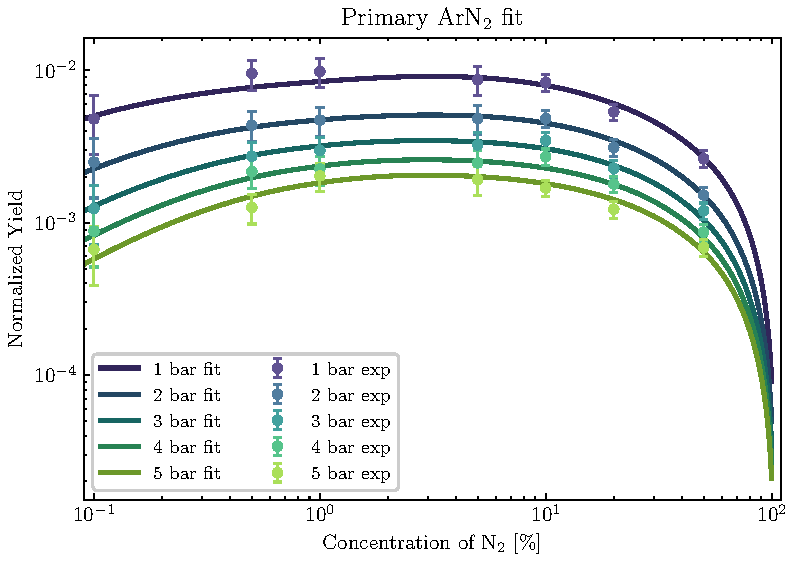
\includegraphics[width=0.65\linewidth]{primary_fit/ArN2_global.pdf}
    \caption{Ajuste global para la mezcla Ar--N$_2$.}
    \label{fig:ArN2Fit}
\end{figure}

\begin{minipage}{0.45\linewidth}
    \centering
    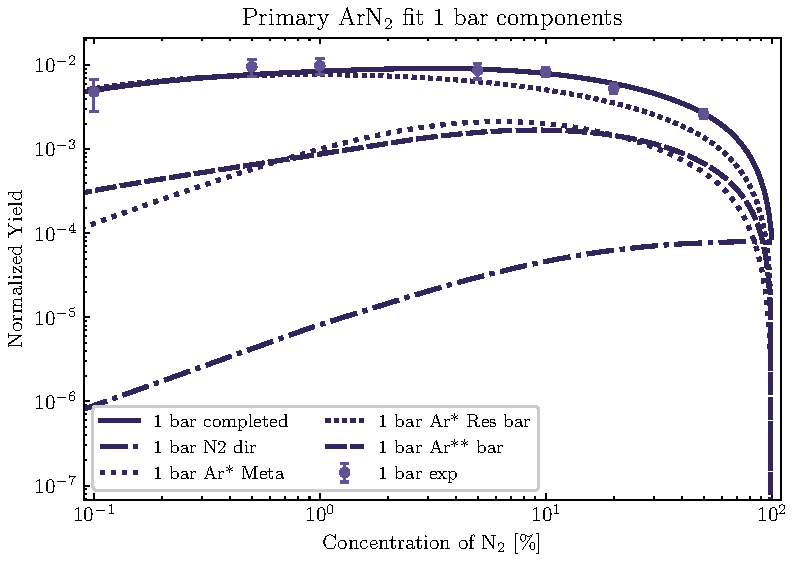
\includegraphics[width=0.99\linewidth]{primary_fit/ArN2_global_components_1bar.pdf}
    \captionof{figure}{Componentes del ajuste global a 1 bar.}
    \label{fig:ArN2Fit1bar}
\end{minipage}
\hfill
\begin{minipage}{0.45\linewidth}
    \centering
    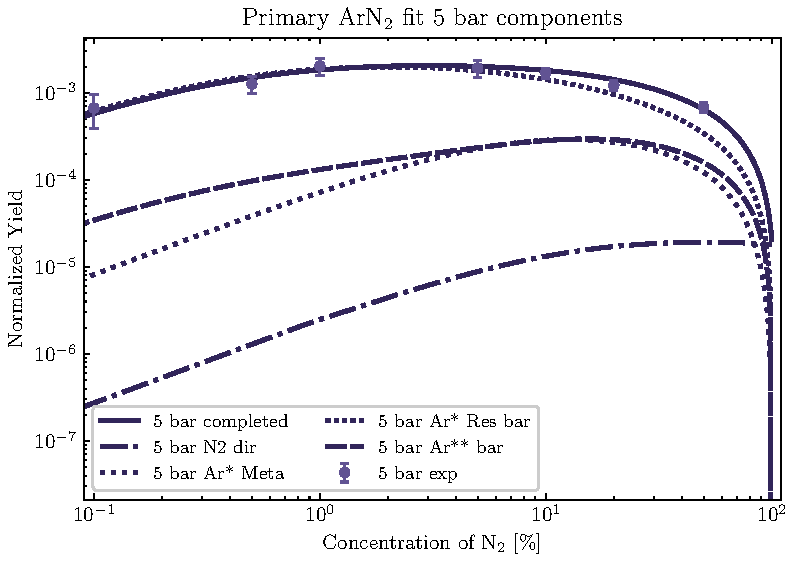
\includegraphics[width=0.99\linewidth]{primary_fit/ArN2_global_components_5bar.pdf}
    \captionof{figure}{Componentes del ajuste global a 5 bar.}
    \label{fig:ArN2Fit5bar}
\end{minipage}




\subsection{Ar--N$_2$ en el infrarrojo}

Para la emisión NIR en Ar--N$_2$ se ajusta de forma independiente cada longitud de onda mediante
\begin{equation}
    \frac{Y_{\mathrm{IR},\lambda}}{W_I(f)} = P_{\Ar^*,\lambda} \cdot N_{\Ar^*,\lambda} \cdot \pqty{\frac{1 / \tau_{\Ar^*,\lambda}}{1 / \tau_{\Ar^*,\lambda} + n \cdot f \cdot K_{\Ar^*, Q(\Ar), \lambda} + n \cdot (1-f) \cdot K_{\Ar^*, Q(\N_2), \lambda}} }.
\end{equation}
Aquí $P_{\Ar^*,\lambda}$ incorpora la normalización y la fracción efectiva de estados que alimenta la línea emisora. Las figuras siguientes muestran el ajuste de las líneas NIR consideradas para la mezcla.

\begin{minipage}{0.48\linewidth}
    \centering
    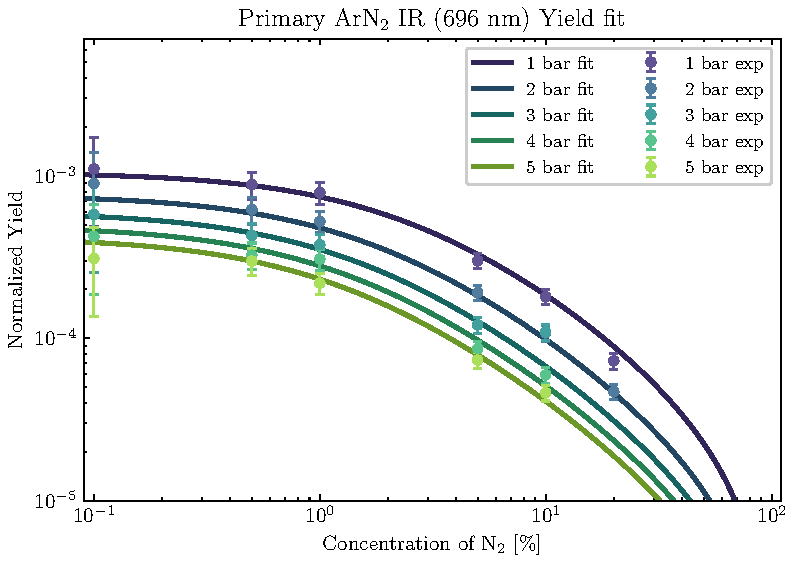
\includegraphics[width=0.99\linewidth]{primary_fit_IR/ArN2_global_696.pdf}
    \captionof{figure}{Ajuste infrarrojo en 696 nm.}
    \label{fig:ArN2696}
\end{minipage}
\hfill
\begin{minipage}{0.48\linewidth}
    \centering
    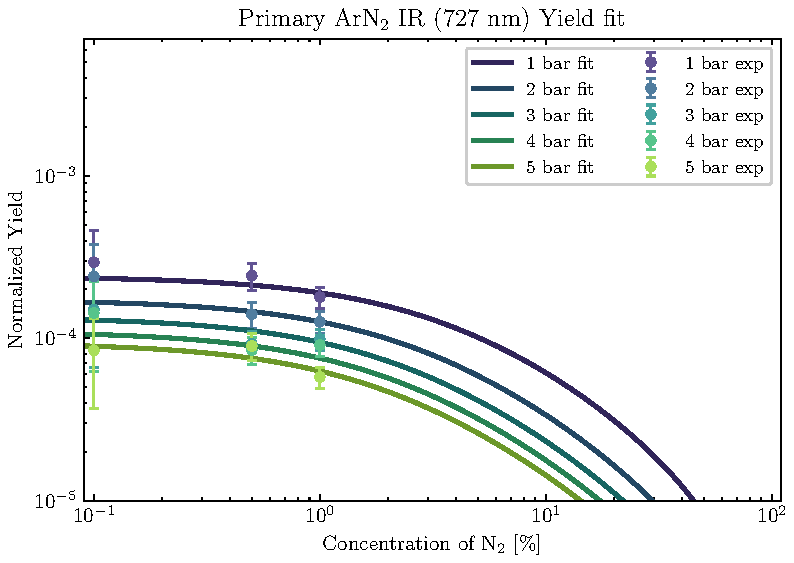
\includegraphics[width=0.99\linewidth]{primary_fit_IR/ArN2_global_727.pdf}
    \captionof{figure}{Ajuste infrarrojo en 727 nm.}
    \label{fig:ArN2727}
\end{minipage}

\begin{minipage}{0.48\linewidth}
    \centering
    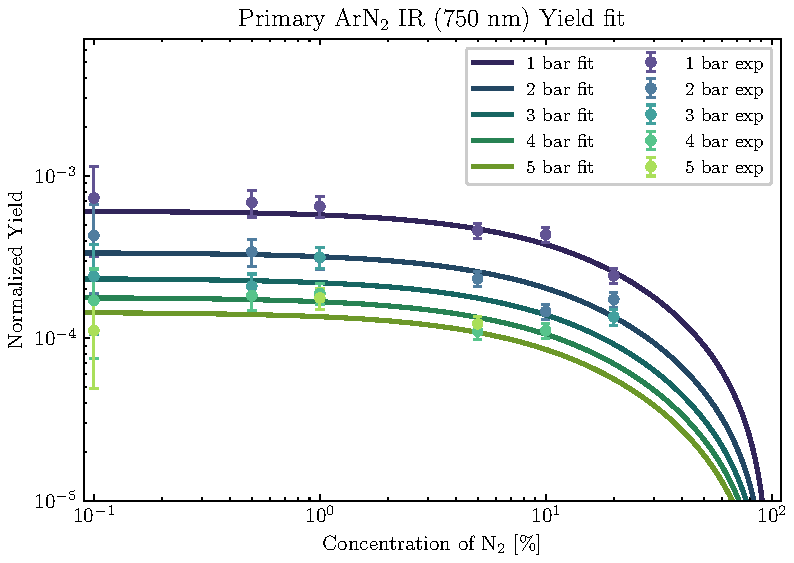
\includegraphics[width=0.99\linewidth]{primary_fit_IR/ArN2_global_750.pdf}
    \captionof{figure}{Ajuste infrarrojo en 750 nm.}
    \label{fig:ArN2750}
\end{minipage}
\hfill
\begin{minipage}{0.48\linewidth}
    \centering
    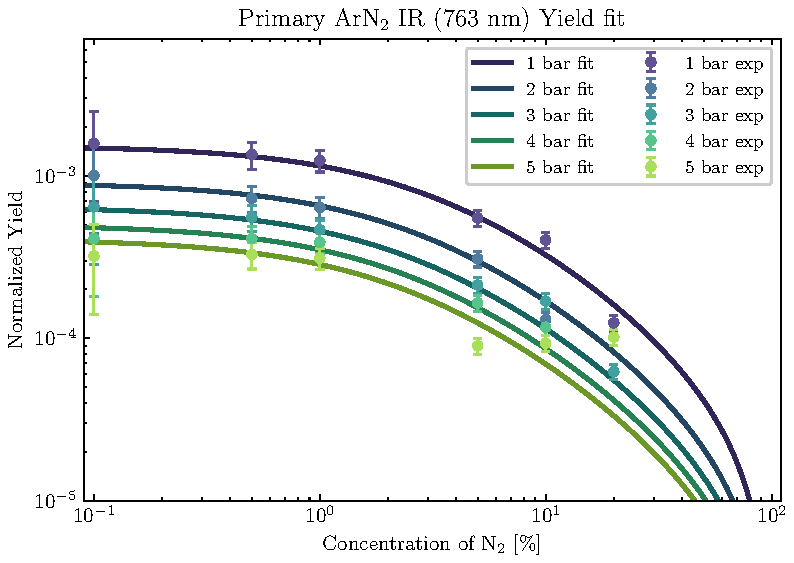
\includegraphics[width=0.99\linewidth]{primary_fit_IR/ArN2_global_763.pdf}    \captionof{figure}{Ajuste infrarrojo en 763 nm.}
    \label{fig:ArN2763}
\end{minipage}

\begin{center}
\begin{minipage}{0.48\linewidth}
    \centering
    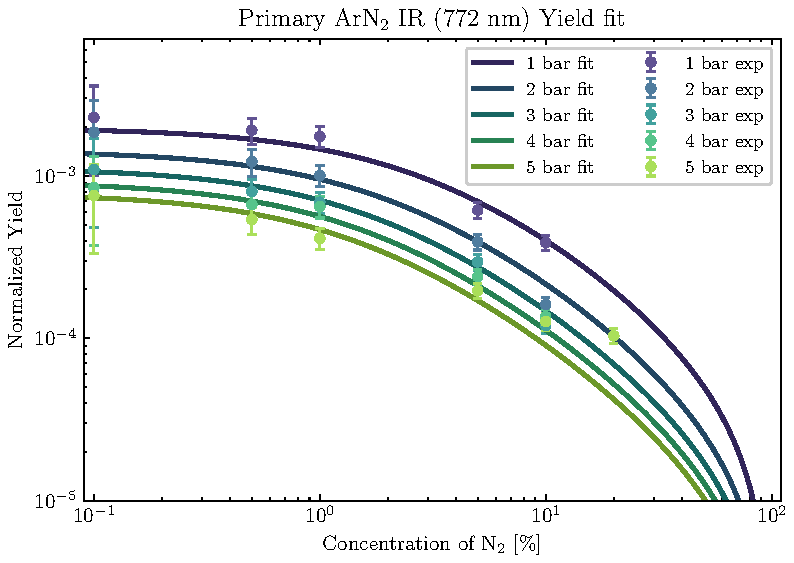
\includegraphics[width=0.99\linewidth]{primary_fit_IR/ArN2_global_772.pdf}
    \captionof{figure}{Ajuste infrarrojo en 772 nm.}
    \label{fig:ArN2772}
\end{minipage}
\end{center}

% =================================================
\section{Predicciones}
% =================================================

Con el modelo cinético de Ar--N$_2$ y los parámetros extraídos del ajuste se obtienen predicciones absolutas del centelleo primario en función de la presión y de la concentración de nitrógeno. Las poblaciones microscópicas de entrada proceden de Degrad para fotones incidentes de 12 keV.

\subsection{Predicciones absolutas ph/MeV}

La figura~\ref{fig:ArN2uvPrimaryPrediction} muestra la predicción UV asociada a la segunda banda positiva del nitrógeno para una amplia variedad de concentraciones a 1 bar. La comparación emplea medidas de centelleo disponibles en la literatura \cite{morii2004quenching,lehaut2015scintillation,colin2007macfly}.

\begin{figure}[h!]
    \centering
    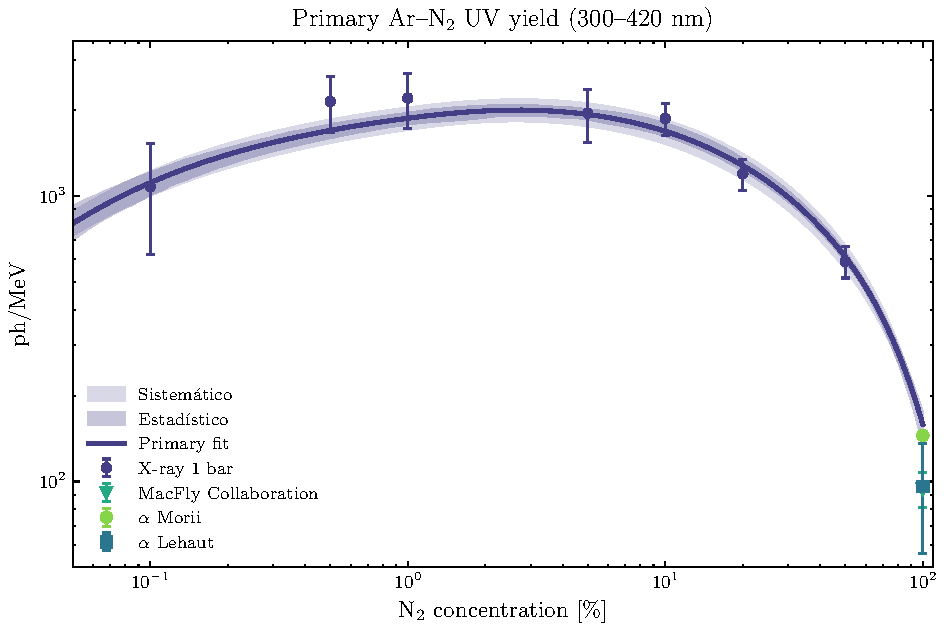
\includegraphics[width=0.70\linewidth]{primary_prediction/ArN2_bands_toy_stat_syst.pdf}
    \caption{Rendimiento de centelleo primario absoluto ultravioleta en $\Ar-\N_2$, comparado con datos experimentales.}
    \label{fig:ArN2uvPrimaryPrediction}
\end{figure}

La figura~\ref{fig:ArN2IrPrimaryPrediction} presenta la predicción absoluta NIR para concentraciones entre 0.01\% y 100\% y presiones de 1 a 5 bar. Esta componente permite cuantificar la supresión de las líneas atómicas del argón al abrirse canales de transferencia y \emph{quenching} por N$_2$.

\begin{figure}[h!]
    \centering
    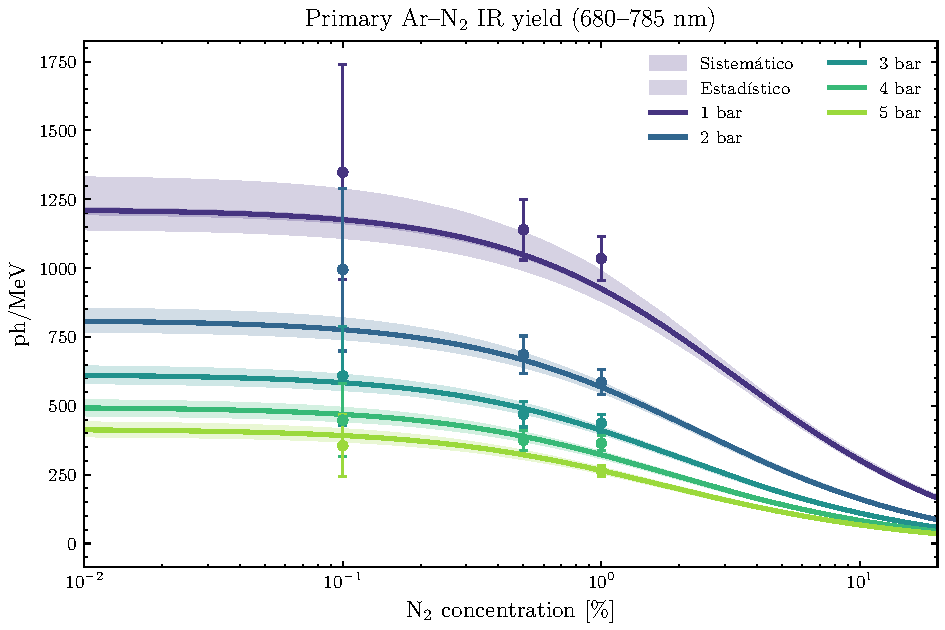
\includegraphics[width=0.62\linewidth]{primary_prediction/ArN2_IR_total_bands_toy_stat_syst.pdf}
    \caption{Rendimiento de centelleo primario absoluto NIR en $\Ar-\N_2$.}
    \label{fig:ArN2IrPrimaryPrediction}
\end{figure}

\subsection{Espectros predichos}

El espectro se reconstruye ponderando cada componente de rendimiento absoluto con una gaussiana centrada en la longitud de onda de la transición correspondiente:
\begin{equation}
    Y(\lambda, f_{\N_2}, p) = \sum_i Y_i(f_{\N_2}, p)\, \mathrm{gauss}(\lambda;\, \mu=\lambda_i,\sigma=\sigma_i).
\end{equation}

\begin{figure}[h!]
    \centering
    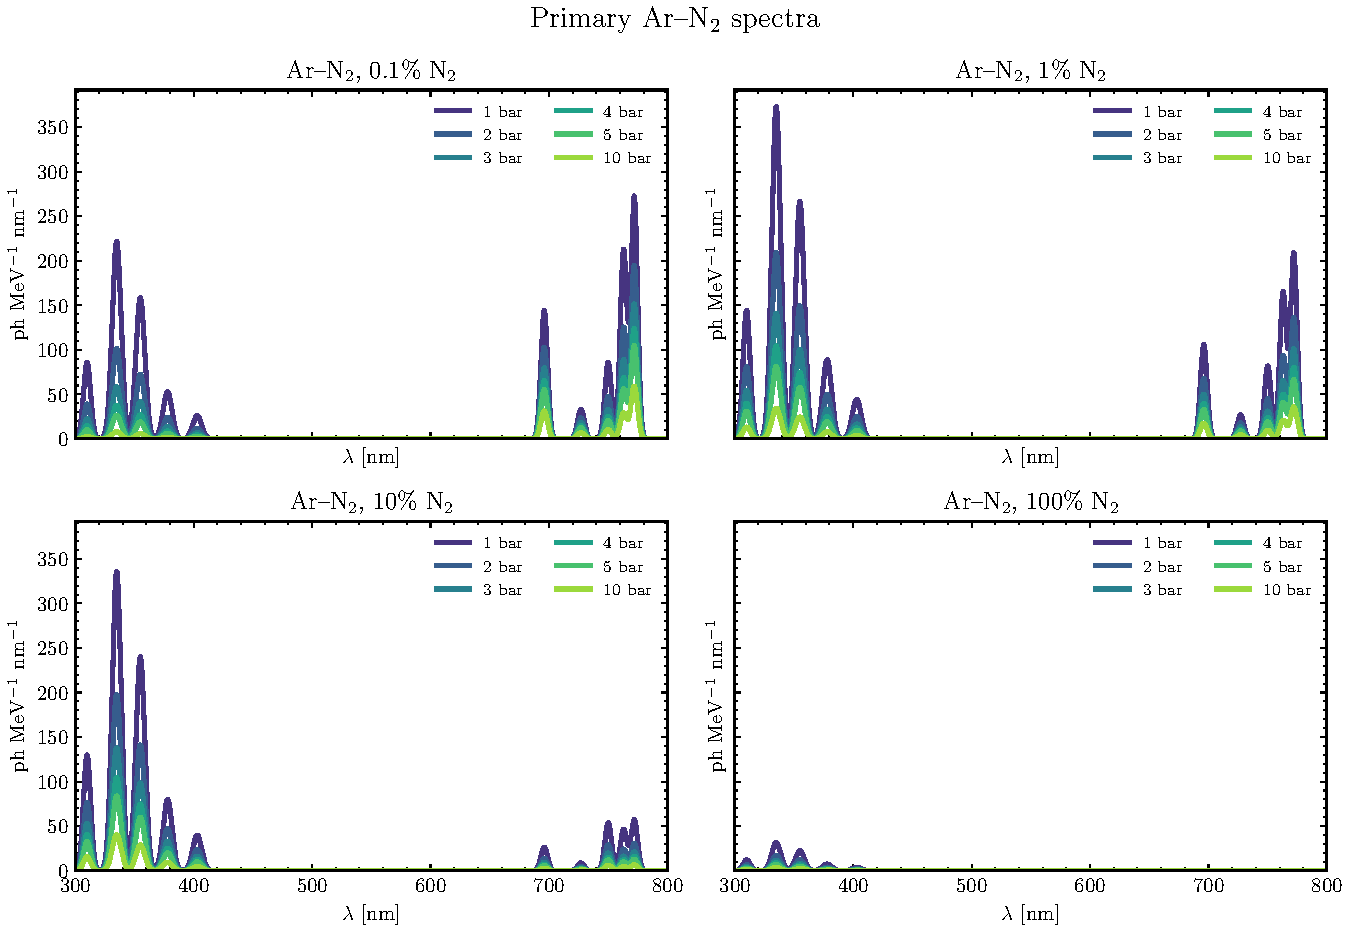
\includegraphics[width=0.9\linewidth]{predicted_spectra/ArN2_concentration_ph_MeV_nm.pdf}
    \caption{Espectros de $\Ar-\N_2$ predichos en función de la concentración y de la presión en el rango 200--800 nm.}
    \label{fig:ArN2PrimarySpectra}
\end{figure}


% =================================================
\section{Conclusiones}
% =================================================

En este trabajo se ha desarrollado una descripción fenomenológica del centelleo primario de la mezcla $\Ar-\N_2$ para lectura óptica en detectores gaseosos. El modelo separa la producción microscópica de poblaciones excitadas, calculada con Degrad, de su evolución cinética mediante transferencia energética, emisión radiativa y \emph{quenching}. Esta estrategia permite conectar las colisiones electrón--gas con rendimientos ópticos absolutos en las regiones UV y NIR.

La señal ultravioleta queda dominada por la segunda banda positiva del nitrógeno, $\N_2(\mathrm{C}^3\Pi_u)\rightarrow\N_2(\mathrm{B}^3\Pi_g)$, alimentada tanto por producción directa como por transferencia desde estados excitados del argón. El ajuste global utiliza datos en cinco presiones y ocho concentraciones, y alcanza una compatibilidad satisfactoria con los datos experimentales. La descomposición del rendimiento permite distinguir la diferente dependencia con la presión de las contribuciones asociadas a estados resonantes y metaestables del argón.

La emisión infrarroja ofrece la información complementaria: las líneas NIR del argón se reducen conforme aumenta la concentración de N$_2$, debido a la competencia entre su decaimiento radiativo y los canales colisionales introducidos por el aditivo. El análisis conjunto de UV y NIR muestra así el proceso de conversión espectral de forma directa: la mezcla desplaza señal desde emisiones atómicas del argón hacia bandas moleculares del nitrógeno más accesibles para sensores ópticos convencionales.

Desde el punto de vista instrumental, $\Ar-\N_2$ constituye una mezcla atractiva para MPGDs con lectura óptica por su bajo coste, su sencillez química y la posibilidad de producir emisión UV cercana con pequeñas concentraciones de aditivo. Las predicciones absolutas y los espectros reconstruidos proporcionan una base útil para seleccionar concentraciones y presiones de operación en futuros estudios experimentales.

Como líneas futuras, resulta prioritario contrastar estas predicciones con nuevas medidas absolutas de centelleo en condiciones controladas, extender el modelo al secundario de avalancha en geometrías MPGD realistas y mejorar la identificación microscópica de los estados que alimentan la emisión de $\N_2(\mathrm{C})$. Con estas extensiones podría evaluarse de forma completa la capacidad de $\Ar-\N_2$ como mezcla de lectura óptica para detectores gaseosos de gran volumen.

% =================================================

\printbibliography
\addcontentsline{toc}{section}{Referencias}

\end{document}
